\documentclass[Orbiter User Manual.tex]{subfiles}
\begin{document}

\section{Extra functionality}
\label{sec:extra}
The standard Orbiter installation comes with a set of optional plug-in modules which can be used to enhance the core functionality of the simulator. To enable these additional functions, the appropriate modules must be loaded in the \textit{Modules} tab of the Orbiter Launchpad dialog (see \ref{ssec:launchpad_modules} on how to activate plug-in modules).\\
Many more plug-ins are available from 3$^{rd}$ party add-on developers. Check out the Orbiter repositories on the web to find more.\\
You should only activate modules you want to use during your simulation session, because many plug-ins may consume CPU cycles even if they are running in the background. Too many active modules can degrade the simulation performance.\\
When activated, some plug-ins, such as custom MFD modes, take effect automatically whenever the simulation is started. Others are accessible via the \textit{Custom functions} dialog (see \ref{ssec:menu_cust_func}).


\subsection{Scenario editor}
\label{ssec:scn_editor}
Orbiter's \textit{Scenario Editor} can be used to create, configure and delete vessels during a running simulation session.

\begin{figure}[H]
	\centering
	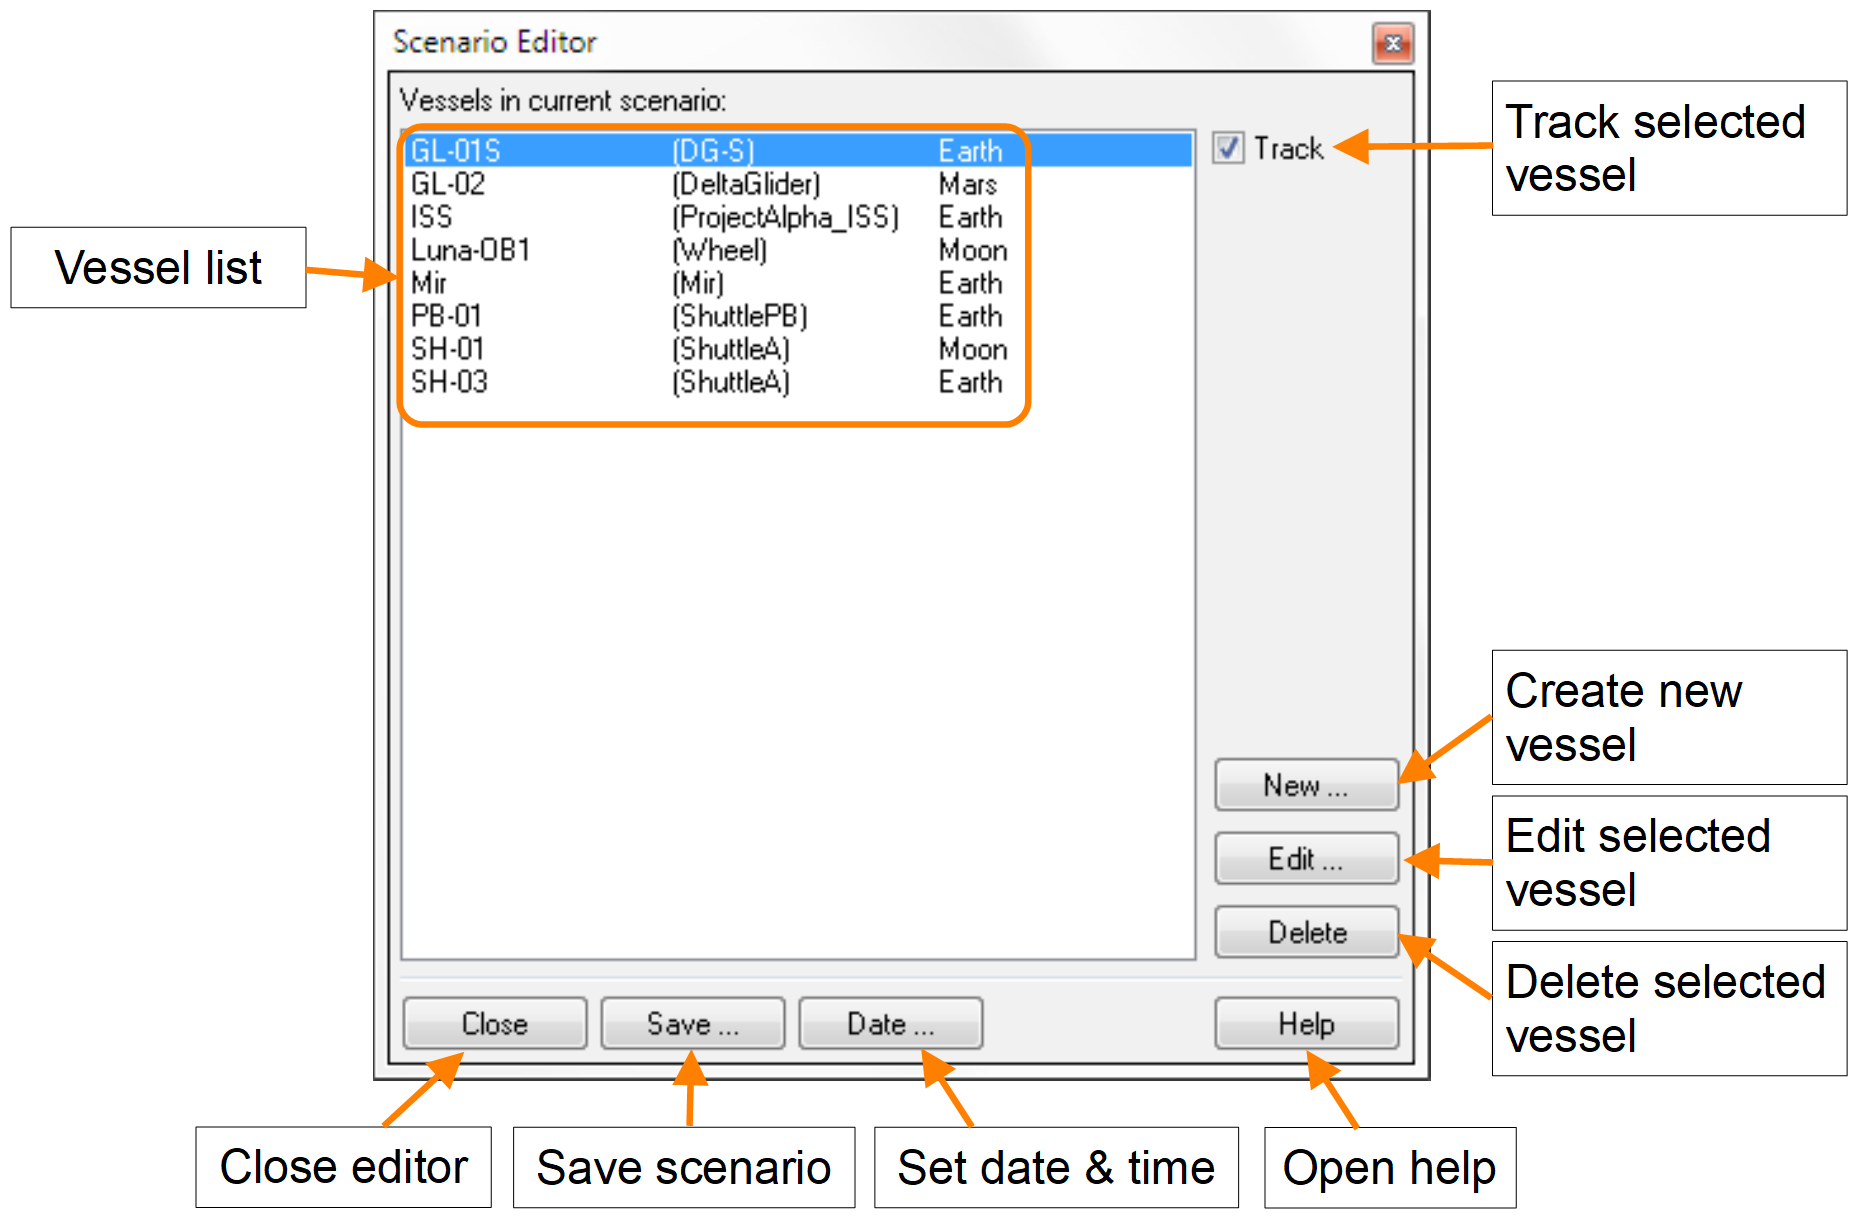
\includegraphics[width=\hsize]{scn_main.png}
\end{figure}

\noindent
Vessel states can be edited by applying orbital elements, state vectors, surface location, fuel states, docking connections or vessel-specific parameters. The resulting configuration can be saved as a scenario and used to launch a simulation session later.\\
The editor is provided as a plug-in module that comes with the default Orbiter installation. To make it available in Orbiter, make sure that the ScnEditor module is loaded from the \textit{Modules} tab of the Orbiter Launchpad dialog (see \ref{ssec:launchpad_modules}).\\
During the simulation, the scenario editor can be opened from the list in the \textit{Custom Functions} dialog (\Ctrl\keystroke{F4}). This brings up the editor's main page, containing a list of all vessels in the current simulation session. Each entry displays the vessel name, class and reference celestial body. When a vessel is selected from the list, the camera automatically jumps to that vessel if the \textit{Track} box is ticked.\\
From the main page, the user has the option to

\begin{itemize}
\item create a new vessel,
\item edit the vessel selected in the list,
\item delete the selected vessel,
\item change the simulation date, or
\item save the scenario to a file.
\end{itemize}


\subsubsection{Creating a new vessel}
After clicking the \textit{New} button on the main page, the editor displays the vessel creation page. It shows a list of all spacecraft types recognised by Orbiter in the \textit{Vessel} type box. Note that some vessel types may be located in subfolders. To see what a particular vessel class looks like, click on the entry in the list, and a picture is shown next to it. (Not all vessel types may support this feature).

\begin{figure}[H]
	\centering
	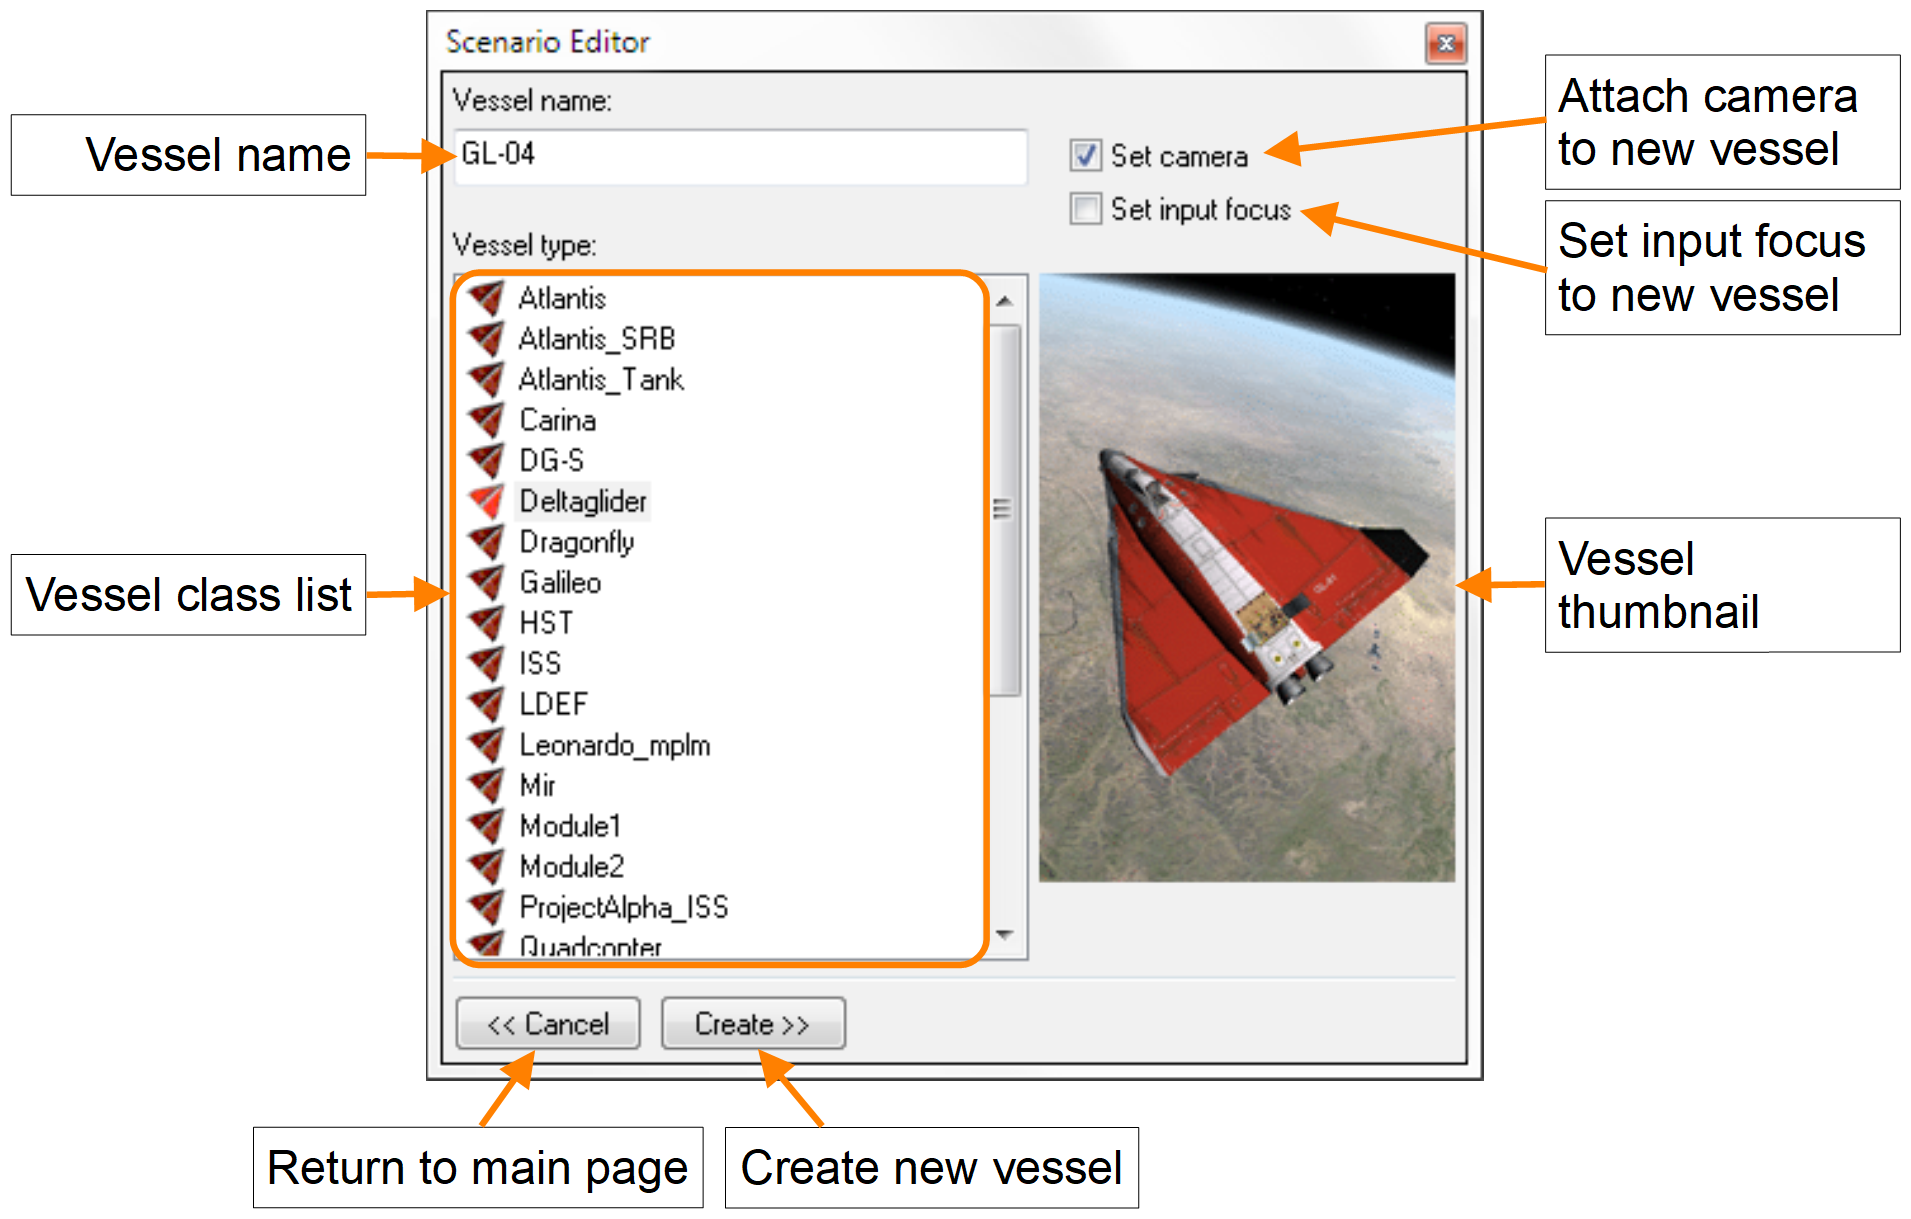
\includegraphics[width=\hsize]{scn_new.png}
\end{figure}

\noindent
Select a type from the list, and enter a unique vessel name in the \textit{Vessel name} box above. If you enter a name that is already in use, or forget to select a vessel type, the editor will not allow you to proceed.\\
If you want the simulator to display the new vessel as soon as it is created, tick the \textit{Set camera} box. In addition, ticking the \textit{Set input focus} box makes the new vessel the focus vessel, receiving user input via keyboard, mouse and joystick. Note that some vessel types may not accept input focus.\\
Click the \textit{Create} button to generate the new vessel. All new vessels are placed in a default location (in a low Earth orbit).\\
The editor now switches to Configuration mode. From here, the position, orientation and other state parameters of the new vessel can be set.


\subsubsection{Configuring a vessel}
After clicking the Edit button on the main page, or after creating a new vessel, the scenario editor displays the vessel configuration page for the selected vessel. From here, various aspects of the vessel state can be adjusted, such as its position, velocity and orientation. It can also be refuelled or docked to another vessel. Some vessel types may also allow control of class-specific parameters from here (see "Scenario Editor" in Orbiter Developer Manual).\\
\textbf{Note:} Although not strictly necessary, it is sometimes useful to pause the simulation (\Ctrl\keystroke{P}) before editing a vessel. Otherwise the continuously changing state values may make a precise configuration tricky.

\begin{figure}[H]
	\centering
	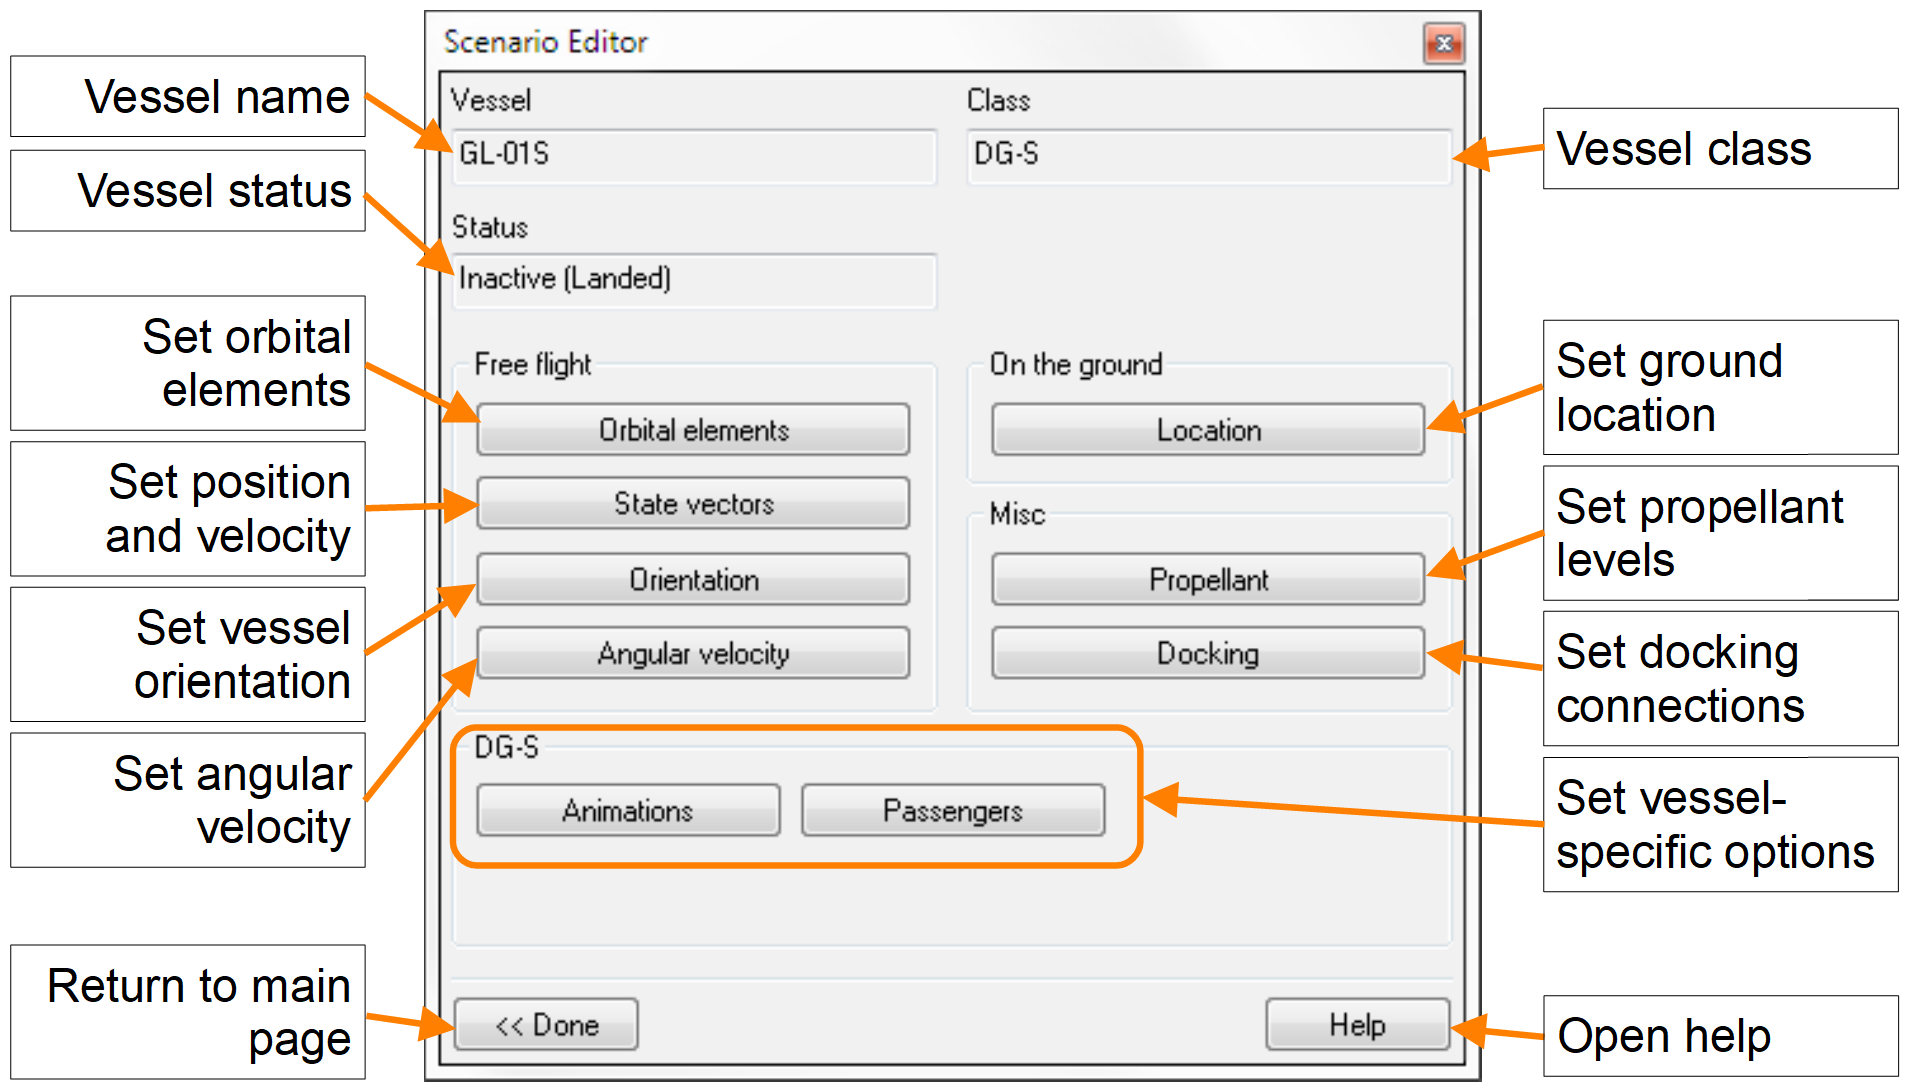
\includegraphics[width=\hsize]{scn_edit.png}
\end{figure}

\subsubsection{Orbital elements}
This page can be used to place a vessel in orbit around a celestial body.

\begin{figure}[H]
	\centering
	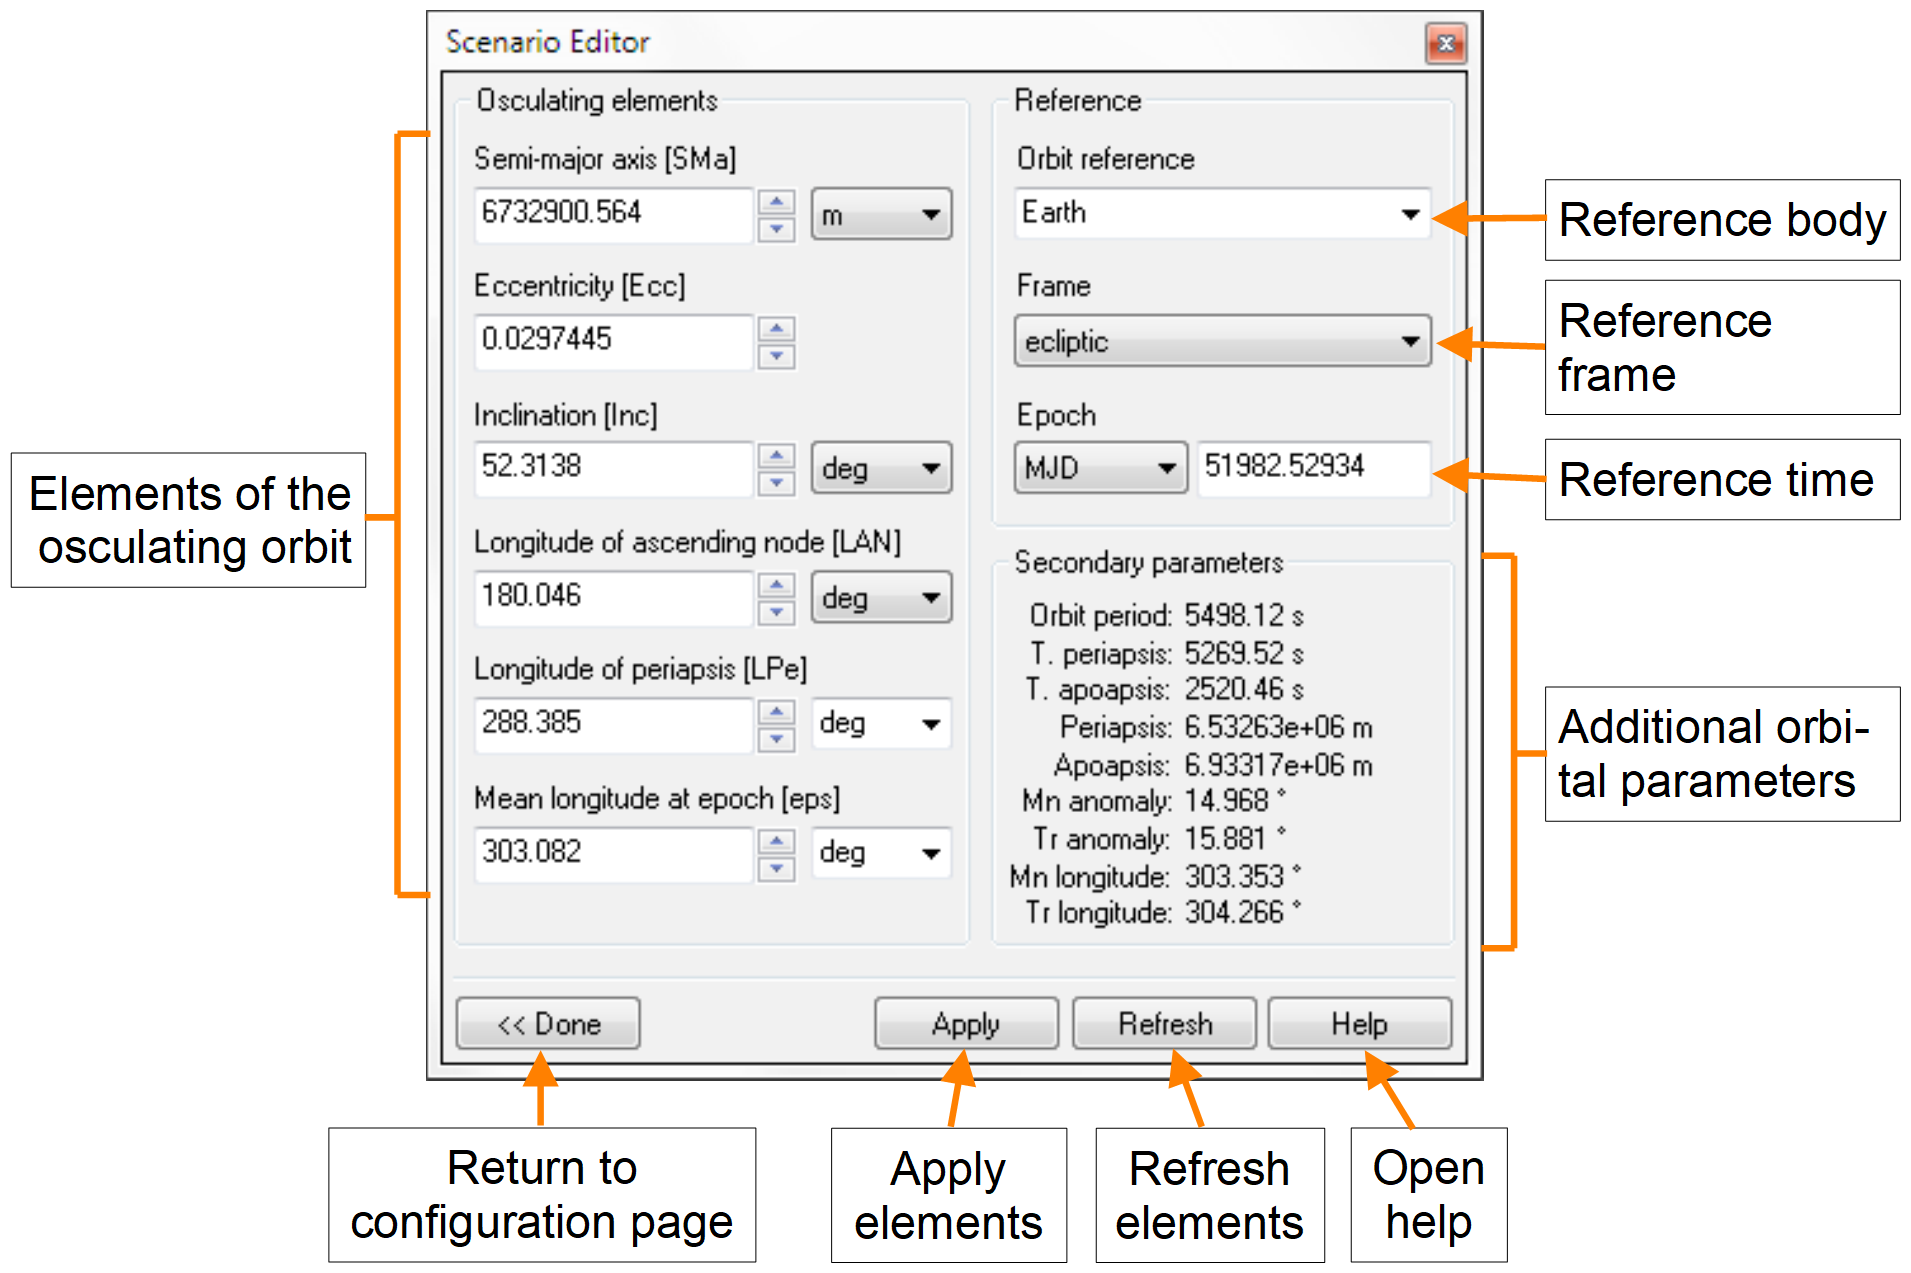
\includegraphics[width=\hsize]{scn_element.png}
\end{figure}

\noindent
First select the reference body (planet, moon or sun) around which the vessel is to orbit in the \textit{Orbit reference} box in the right column.\\
Next, in the \textit{Frame} box below, select the coordinate frame in which the elements are expressed. The choices are \textit{ecliptic} and \textit{ref. equator}. The ecliptic frame is defined by the plane of Earth's orbit and the direction of the vernal equinox (at epoch J2000.0). This frame is useful for example to place the vessel into an orbit for an interplanetary transfer. The equatorial frame is defined by the equatorial plane of the reference body. It is useful if you want to place the vessel into a specific orbit with respect to the planet surface, e.g. geostationary or polar.\\
Finally, set the \textit{reference epoch} for the elements. This is the date to which the \textit{mean longitude} parameter of the orbital elements refers (see below). When setting this to \textit{current}, the longitude value refers to the current simulation time. Otherwise, the value refers to the longitude at the specified MJD (Modified Julian Date). The latter option is more useful when editing a scenario without pausing, because a vessel's mean longitude is continuously changing along its orbit.\\
Now everything is ready to set the elements in the left column. The six elements completely describe a Keplerian (2-body) orbit of an object in the form of a conic section, either periodic (elliptic) or non-periodic (hyperbolic). Under the influence of gravitational perturbations the  elements change over time. In this case, the specified values define the current osculating orbit, i. e. the hypothetical unperturbed orbit that would produce the vessel's state vectors (position and velocity) at the current time.\\
Below is a short description of the 6 orbital elements. See \ref{ssec:sol_orb_mech}.

\paragraph{Semi-major axis [SMa]}
For elliptical orbits, this is the largest semi-diameter of the orbital trajectory. For hyperbolic orbits, SMa is negative and its absolute value represents the distance between the origin (the point where the asymptotes of the hyperbola intersect) and the orbit periapsis.

\paragraph{Eccentricity [Ecc]}
The eccentricity \textit{e} defines the shape of the orbit.

\begin{itemize}
\item e = 0: circular orbit
\item 0 < e < 1: elliptic orbit
\item e = 1: parabolic orbit
\item e > 1: hyperbolic orbit
\end{itemize}

\paragraph{Inclination [Inc]}
Inclination \textit{i} is the angle between the orbital plane and the reference plane. For example, in the equatorial frame, \textit{i} = 0° puts the vessel into an orbit above the planet's equator, while \textit{i} = 90° defines a polar orbit.

\paragraph{Longitude of ascending node [LAN]}
This is the angular distance between the reference direction (e.g. to the vernal point) and the direction to the \textit{ascending node} (the point at which the orbital trajectory passes through the reference plane from below).

\paragraph{Longitude of periapsis [LPe]}
The sum of LAN and the \textit{argument of periapsis} (the angle between the direction to the ascending node and the direction to periapsis).

\paragraph{Mean longitude at epoch [eps]}
This parameter defines the vessel's position along the orbital trajectory. The mean longitude is the sum of LAN and the \textit{mean anomaly} (the angle between periapsis and the vessel position for a hypothetical circular orbit with the same orbital period as the true orbit). The value entered here refers to the specified epoch. For epoch = current, the value represents the vessel's current (continuously varying) mean longitude. Otherwise, it is the longitude at the specified date (fixed for a given orbit).

\subsubsection{State vectors}
Instead of defining the vessel's orbital trajectory by setting its osculating elements as described in the previous section, it is also possible to fix the vessel's \textit{state vectors} (position and velocity) at the current simulation time. Both methods are equivalent, but each may be better suited to specific situations.\\
First, select the desired celestial body (sun, planet or moon) in the \textit{Orbit reference} box. All position and velocity parameters are interpreted relative to the centre of this body.\\
Next, select the reference coordinate frame in which the state vectors are expressed. The \textit{Frame} box provides three options:

\begin{itemize}
\item \textbf{ecliptic:} The ecliptic frame uses the Earth's mean orbital plane (epoch J2000.0) as reference plane (xz), and the direction of the vernal point as reference direction (+x). The ecliptic north pole defines the +y direction.
\item \textbf{ref. equator (fixed):} The frame is defined by the equatorial plane of the reference body (xz), with +y pointing to the north pole. The frame is non-rotating, i.e. fixed with respect to the celestial sphere.
\item \textbf{ref. equator (rotating):} This equatorial frame rotates with the celestial body (around the y-axis). The +x direction points to the prime meridian (longitude 0°).
\end{itemize}

\noindent
Finally, select the coordinates to use. The choice is between cartesian coordinates (\textit{x}, \textit{y}, \textit{z}) and (d\textit{x}/d\textit{t}, d\textit{y}/d\textit{t}, d\textit{z}/d\textit{t}) and spherical polar coordinates (\textit{r}, $\phi$, $\theta$) and (d\textit{r}/d\textit{t}, d$\phi$/d\textit{t}, d$\theta$/d\textit{t}). Generally, polar coordinates will be more intuitive to use.

\begin{figure}[H]
	\centering
	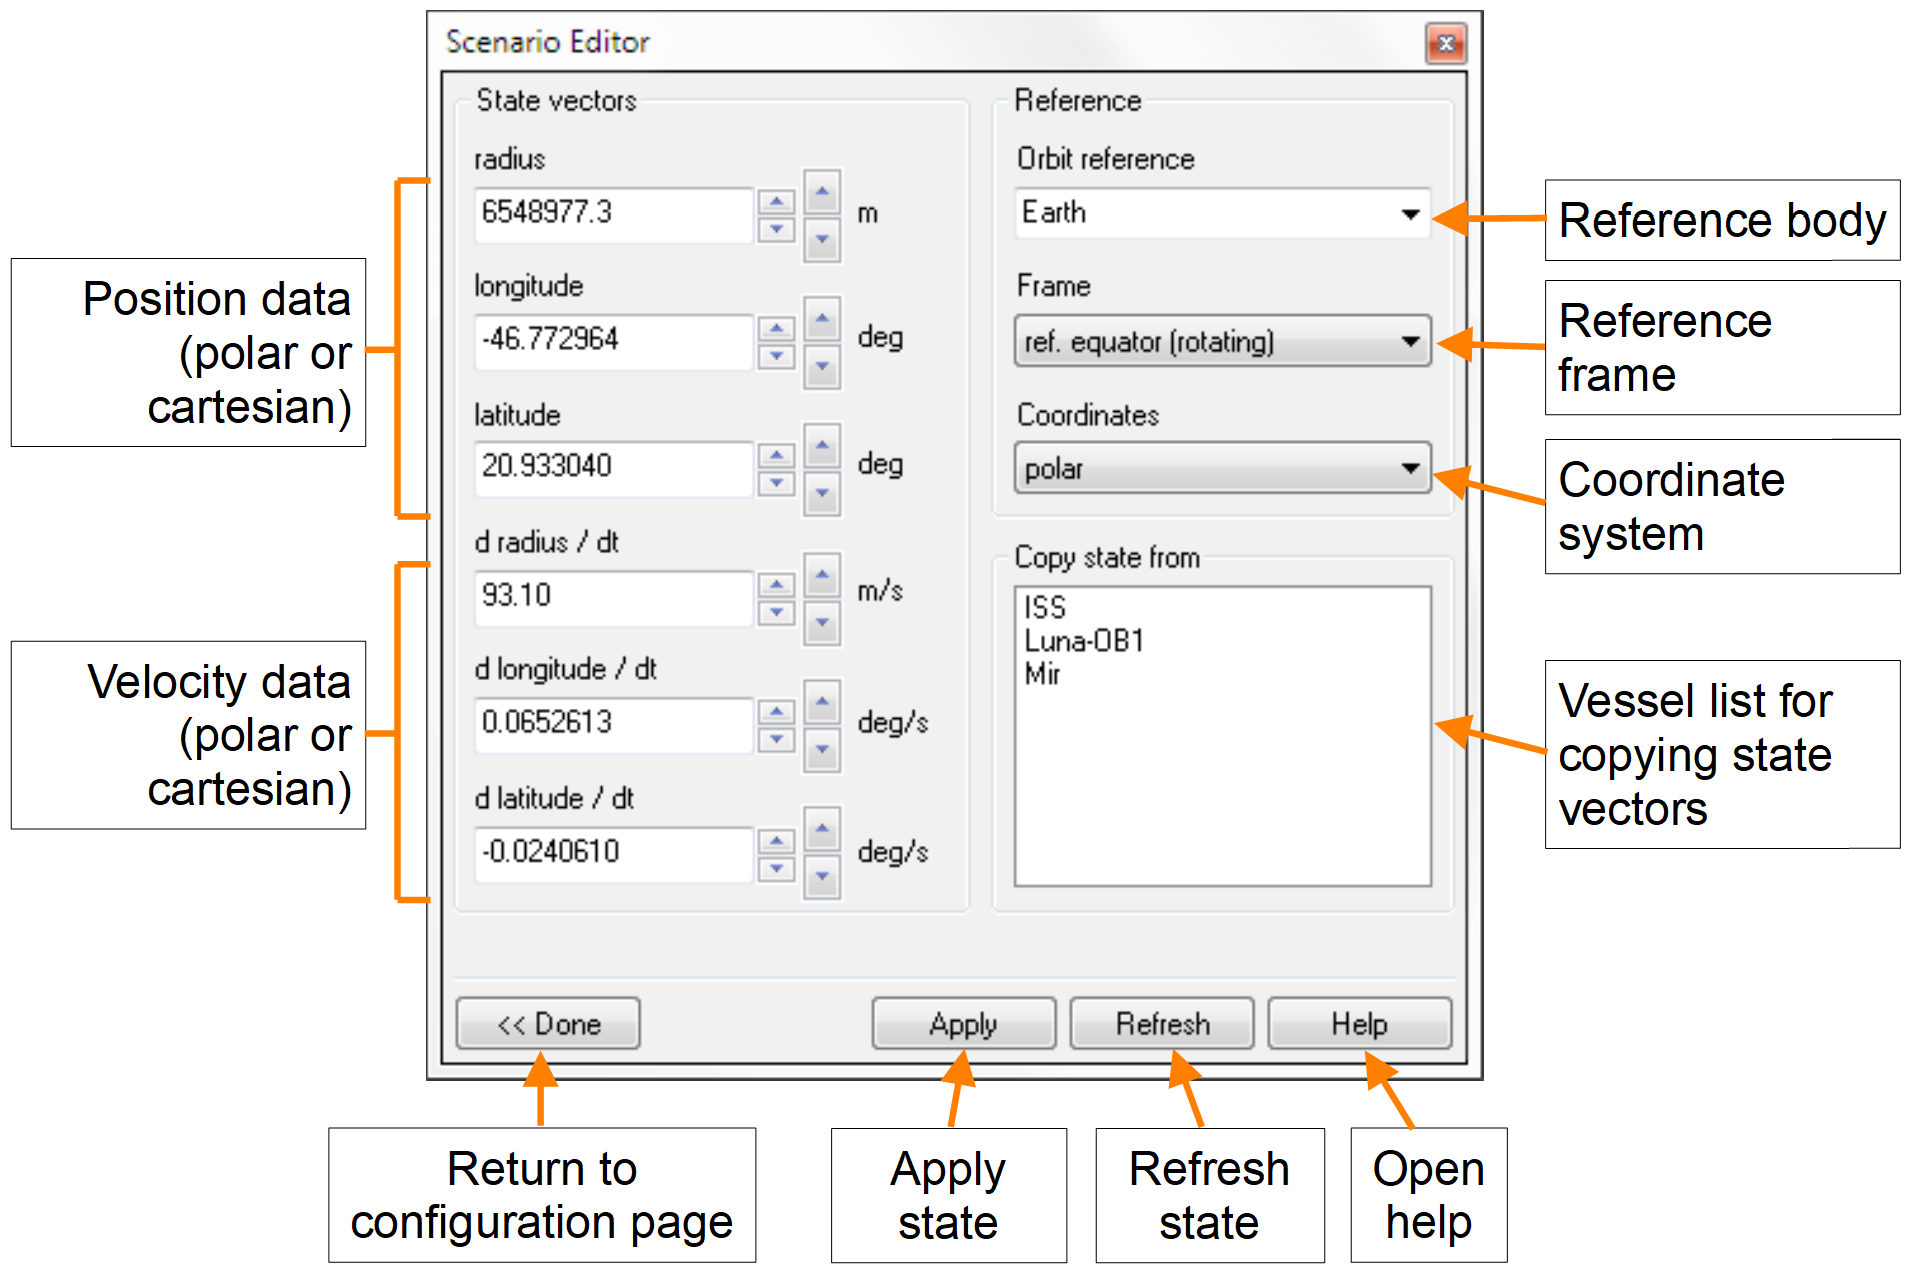
\includegraphics[width=\hsize]{scn_state.png}
\end{figure}

\noindent
Everything is now set to edit the vessel position and velocity values. As the vessel's state vectors are continuously changing during the simulation, it is probably best to pause the simulation at this point. Then press \textit{Refresh} to update the data to the current vessel state. Now enter the new state vector data, and press \textit{Apply} to pass them to the simulation. Use the spin controls next to the input boxes for direct updates.

\paragraph{Copy state}
To place the vessel next to another spacecraft in the simulation, simply copy that vessel's state vectors over into the scenario editor by clicking one of the entries in the \textit{Copy state from} list (Only active vessels are shown in the list). Then click Apply to apply the copied state to your vessel. Unless the simulation was paused, the other vessel may have already moved away in the meantime. To copy and apply the state in a running simulation directly, you can double-click on the vessel in the list.\\
After copying your vessel to the other spacecraft's position, you can edit the state vector entries to fine-tune the relative position and velocity of the two vessels.

\paragraph{Usage tips}
Editing the state vectors is probably most useful when the vessel is close to a planetary surface, for example during atmospheric flight. At orbital altitudes, it is easier to control the vessel state via its orbital elements. Defining a stable orbit via position and velocity data is much more difficult.\\
When editing a vessel close to the surface, the rotating equatorial frame is a good choice. In combination with polar coordinates, the position values translate directly to planetary longitude, latitude and radius data, and the velocity data are equivalent to ground speed in longitudinal, latitudinal and radial direction.\\
By editing its state vectors, the vessel is set to active flight mode. Make sure the parameters you enter define a position above the surface. To place a vessel on the ground, use the \textit{Surface location} page instead.

\subsubsection{Orientation}
Adjust the spacecraft orientation on this page. This applies only to active vessels (in flight), not for landed vessels (whose heading can be adjusted on the \textit{Location} page).\\
Either explicitly set the Euler angles of the spacecraft axes with respect to the ecliptic frame of reference, or rotate the spacecraft around its pitch, yaw and bank axes.

\begin{figure}[H]
	\centering
	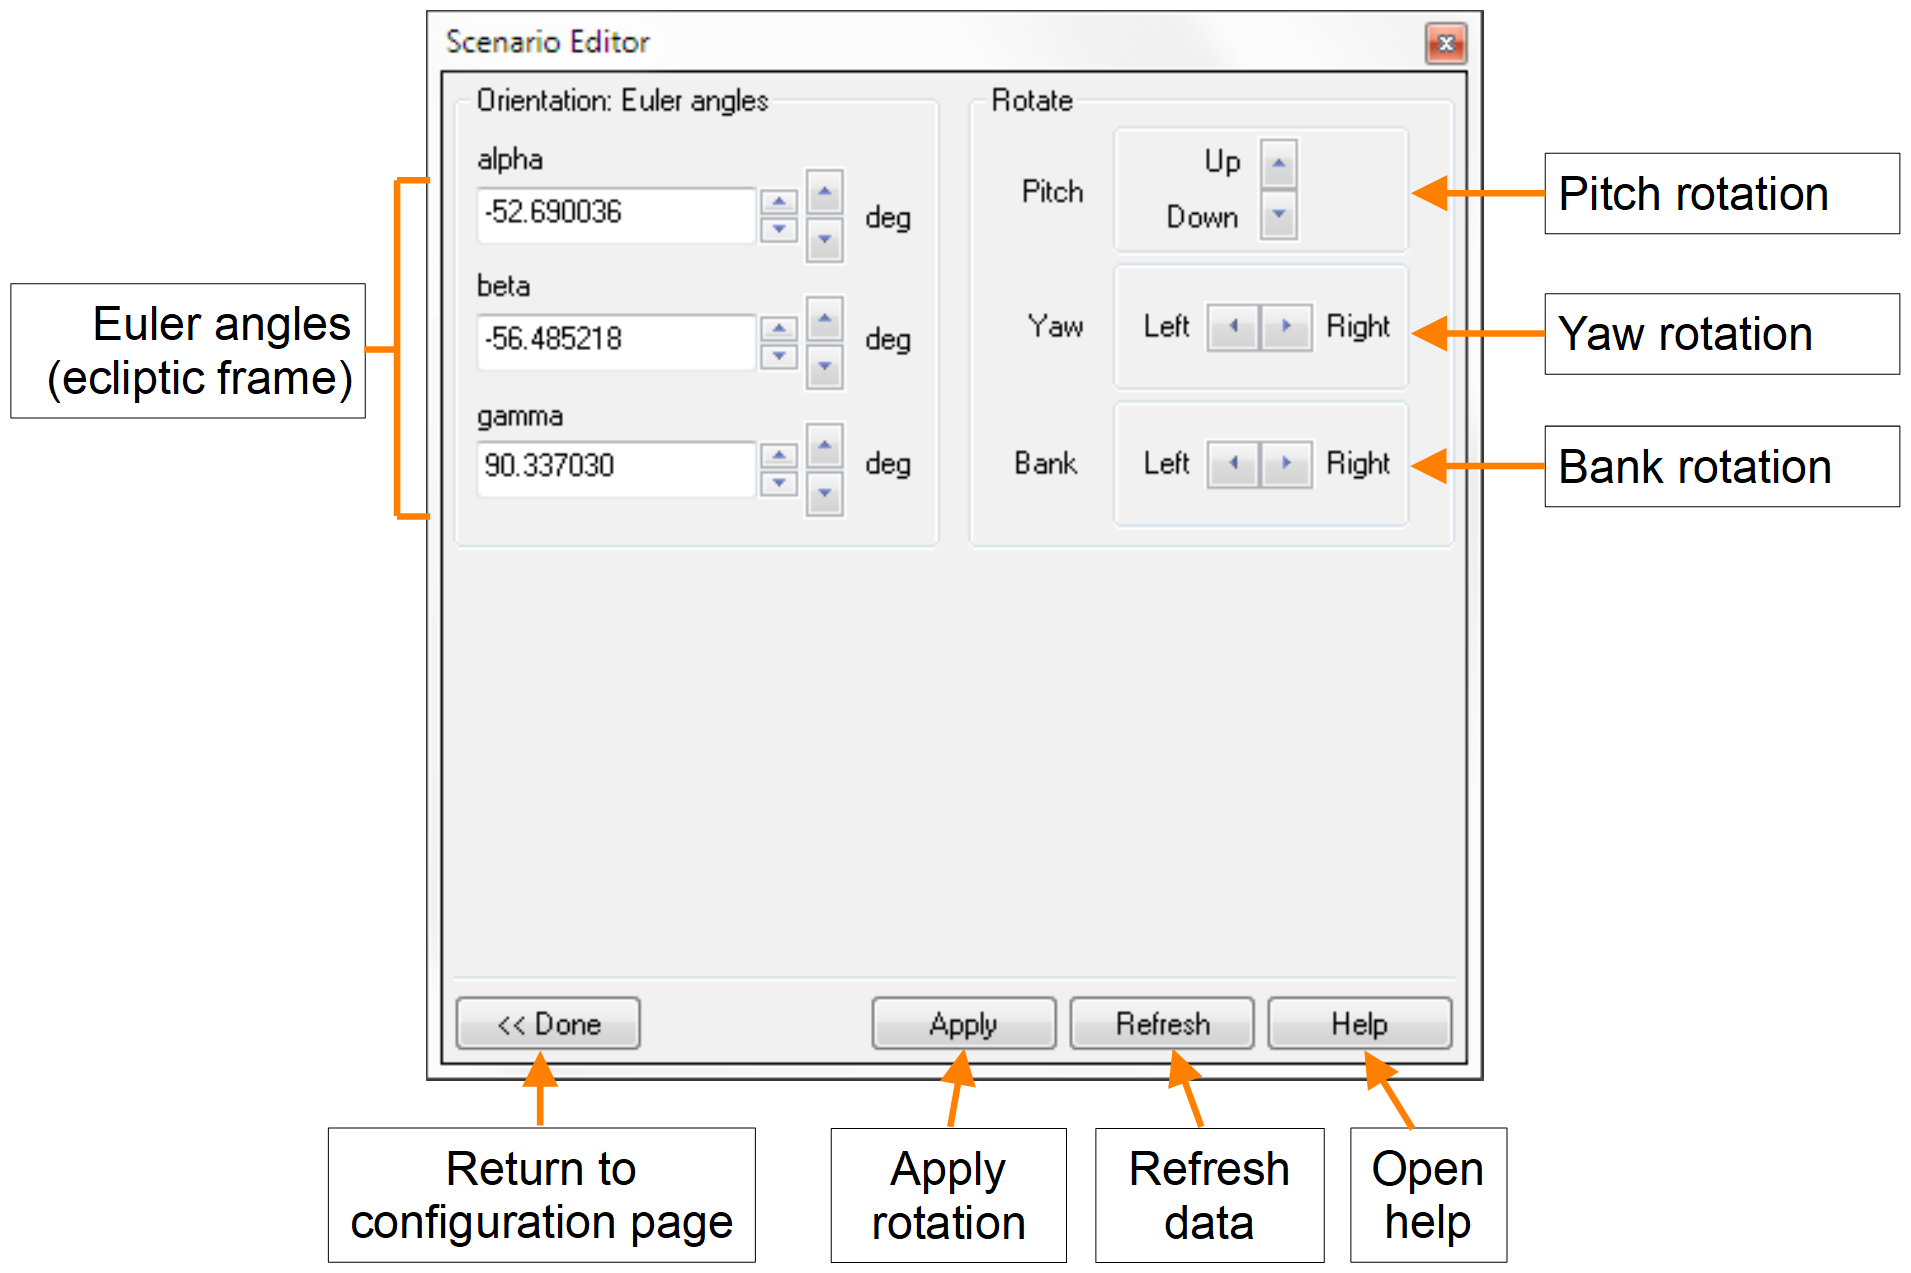
\includegraphics[width=\hsize]{scn_orient.png}
\end{figure}

\noindent
The Euler angles $\alpha$, $\beta$, $\gamma$ define the rotation matrix \textbf{R} which transforms from the vessel local frame to the global ecliptic frame as follows:

\[ \mathbf{R} = 
\begin{bmatrix}
1 & 0 & 0\\
0 & \cos \alpha & \sin \alpha\\
0 & -\sin \alpha & \cos \alpha
\end{bmatrix}
\begin{bmatrix}
\cos \beta & 0 & -\sin \beta\\
0 & 1 & 0\\
\sin \beta & 0 & \cos \beta
\end{bmatrix}
\begin{bmatrix}
\cos \gamma & \sin \gamma & 0\\
-\sin \gamma & \cos \gamma & 0\\
0 & 0 & 1
\end{bmatrix}
\]

\noindent
More intuitively, the vessel can be rotated around its local axes by pressing the pitch, yaw and bank buttons. The pitch buttons rotate the vessel around its x-axis, the yaw buttons around the y-axis, and the bank buttons around the z-axis.\\
If the vessel is part of a composite structure (e.g. a spacecraft docked to a space station), the whole structure will be rotated.

\subsubsection{Angular velocity}
The controls on this page can be used to set the vessel's angular velocity around its three principal axes: x-axis (pitch rate), y-axis (yaw rate) and z-axis (bank rate). To terminate the vessel spin altogether, press the \textit{Kill} button.\\
Note that the angular velocity components can oscillate between the three axes, depending on the vessel's inertia tensor. This means that pressing the Refresh button repeatedly may change the angular velocity values in the three axes, even if no additional torque is applied. Likewise, pressing the Apply button repeatedly with the same angular velocity values can lead to abrupt changes in vessel spin.\\
The angular velocity settings have no effect for vessels on the ground.

\begin{figure}[H]
	\centering
	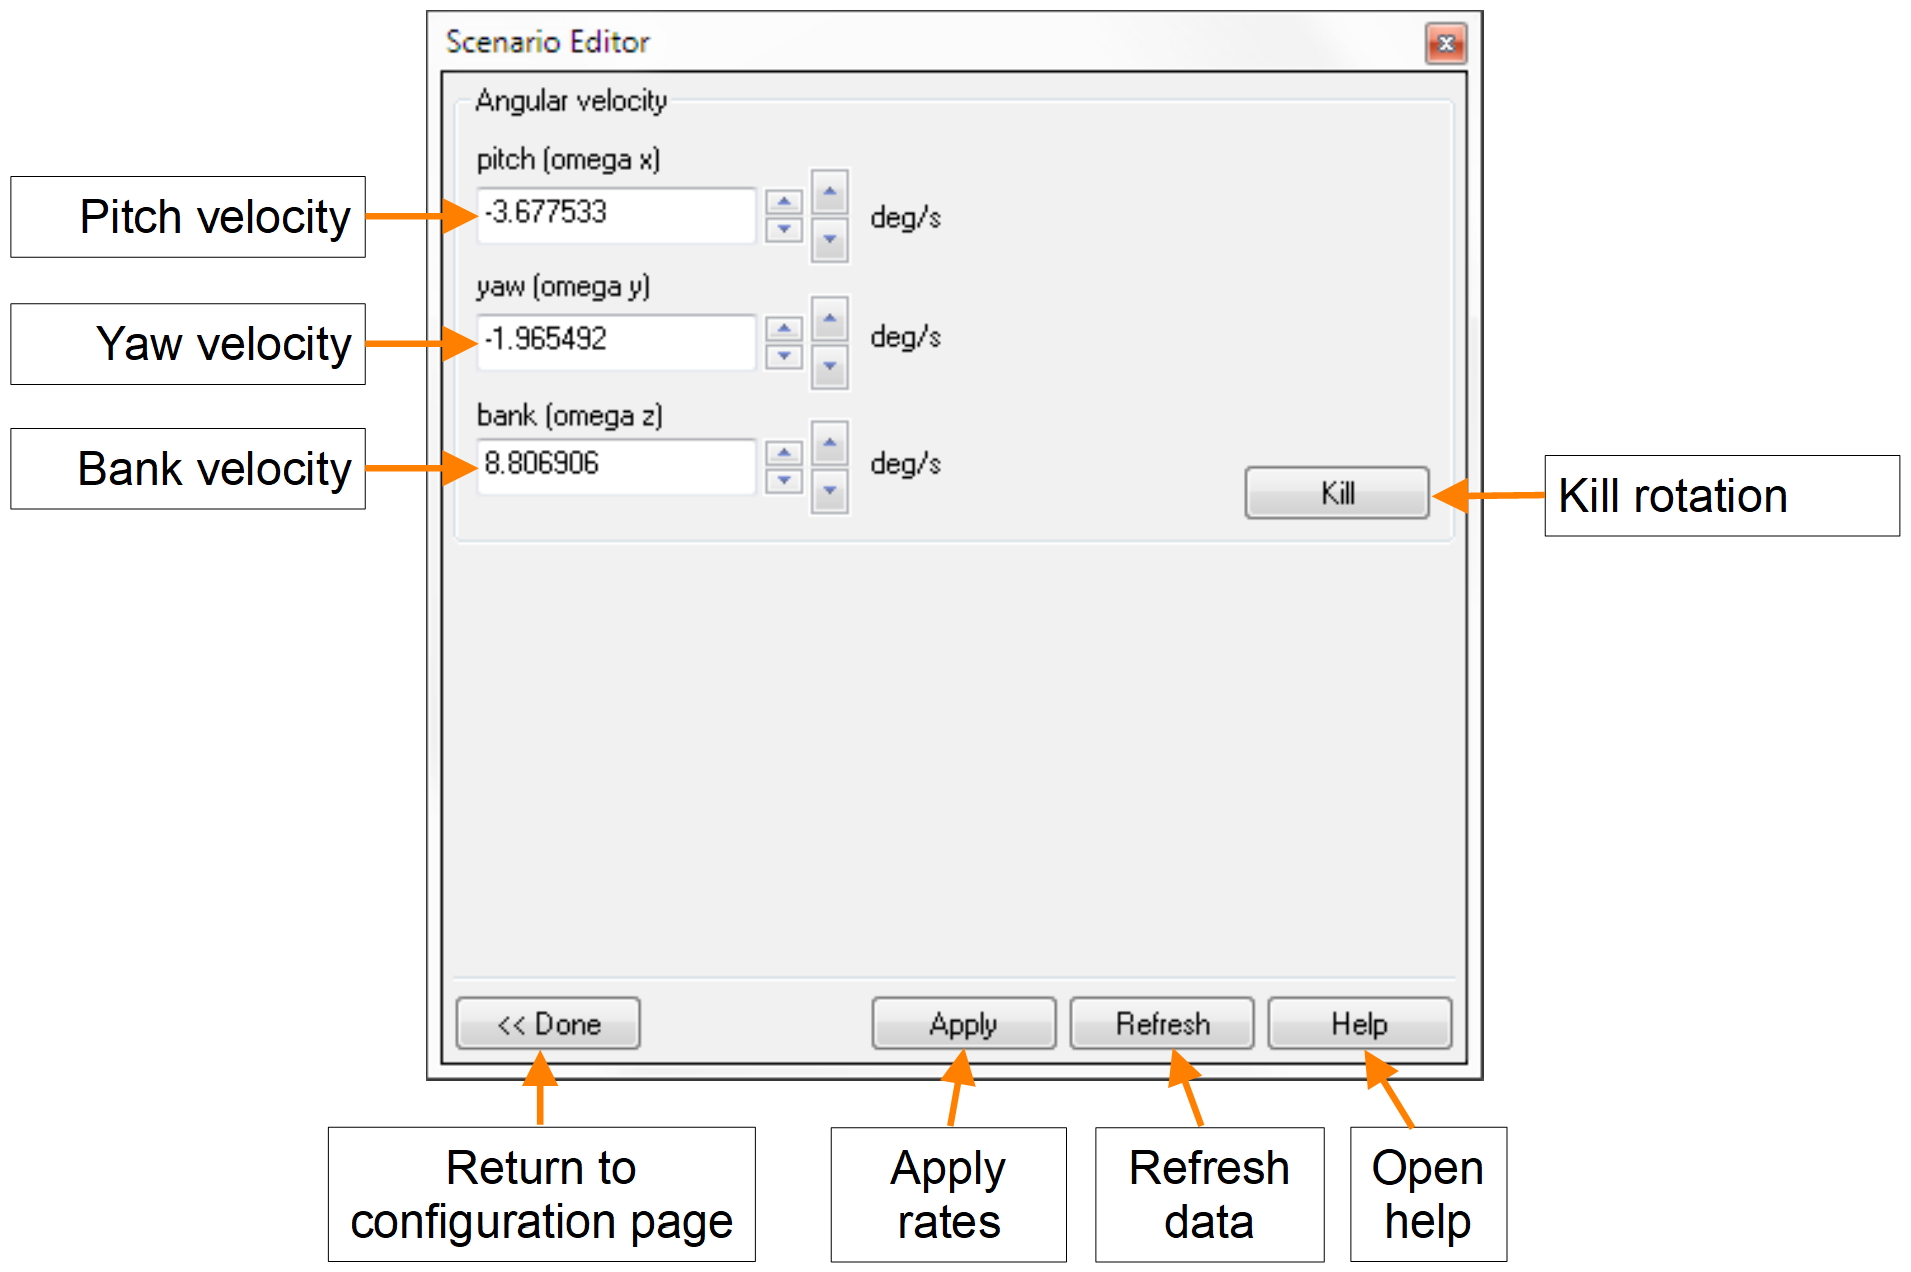
\includegraphics[width=\hsize]{scn_angvel.png}
\end{figure}

\subsubsection{Surface location}
\label{sssec:scneditor_surface}
Applying the options from this page places the vessel on the surface of a planet or moon.\\
First select the body on which to place the vessel in the \textit{Celestial body} box. If applicable, select a spaceport in the \textit{Surface base} box, and a \textit{Landing pad} for the vessel. Alternatively, the equatorial coordinates of the landing site can be input directly in the \textit{Longitude} and \textit{Latitude} boxes. Use the \textit{Heading} box to adjust the orientation of the vessel on the ground.\\
You can use the spin buttons next to the Longitude, Latitude and Heading boxes to adjust the values (small spinners scroll by small amounts, large spinners scroll by large amounts). If numerical values are entered directly, press \textit{Apply} to register the new values.

\begin{figure}[H]
	\centering
	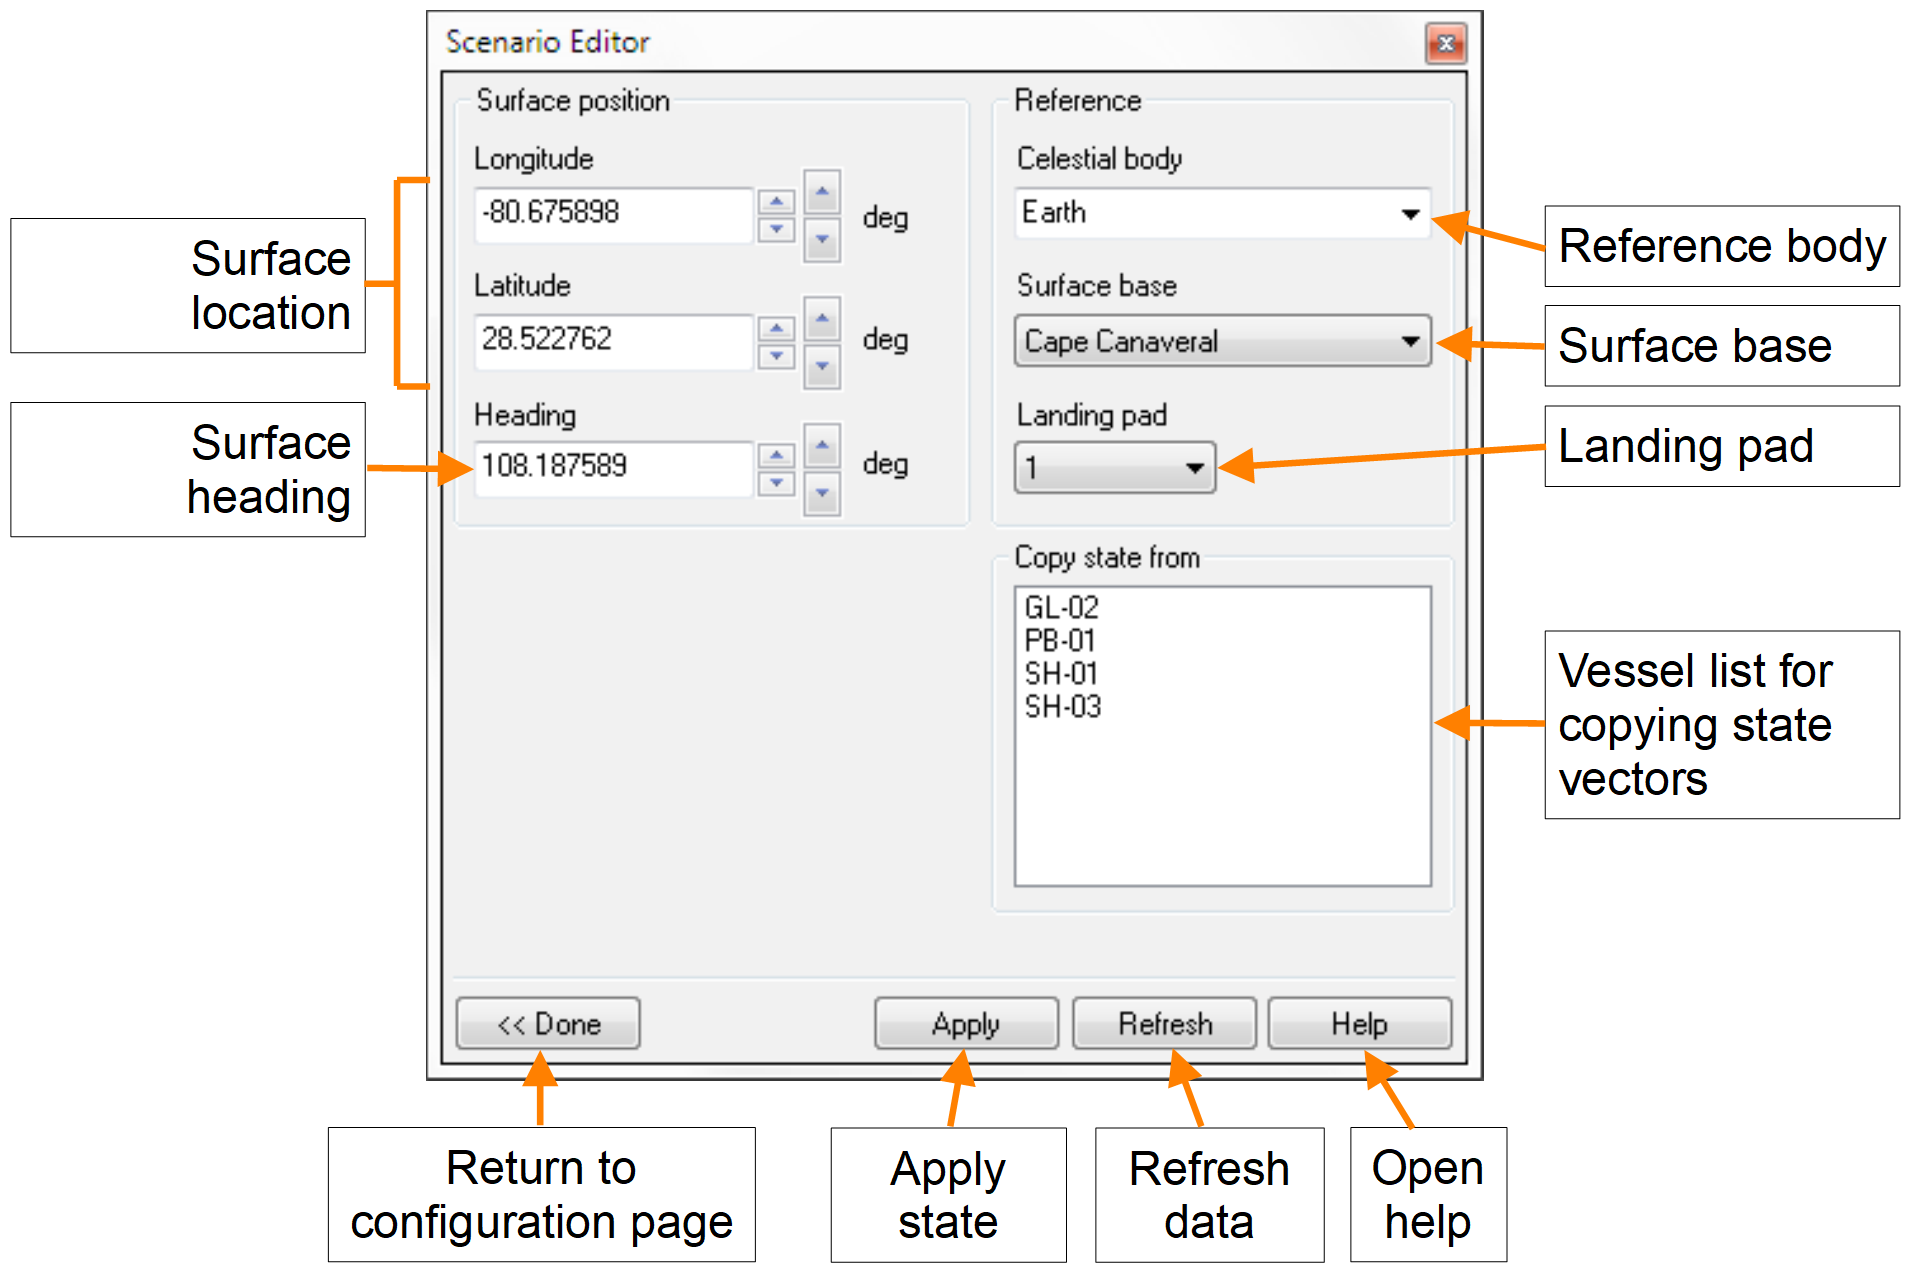
\includegraphics[width=\hsize]{scn_surfloc.png}
\end{figure}

\noindent
\paragraph{Composite structures}
Currently, placing a composite structure of docked vessels on the surface using the scenario editor is not well supported and can lead to positioning artefacts (parts of the structure submerged below the surface or incorrect orientation). To fix a ground-positioning problem, you can try the following workaround:

\begin{itemize}
\item pause the simulation
\item go to the \textit{State vector} tab, switch to rotating equatorial frame and polar coordinates
\item use the radius spinner to lift the composite structure off the ground
\item if necessary, switch to the \textit{Orientation} tab and correct the structure's orientation relative to the ground
\item un-pause the simulation to let the structure drop back to the surface and allow it to settle on its own accord (make sure to start close to the surface, otherwise it will bounce and may fall over before coming to rest).
\end{itemize}

\paragraph{Copy state}
Similar to the State vector page, the Surface location page provides a list of vessels from which the surface parameters can be copied over. All vessels in the list are currently landed on a planetary surface. By clicking on an entry in the list, that vessel's surface parameters are copied into the scenario editor page. You can then click Apply to move your spacecraft to the specified vessel's location. Alternatively, double-clicking applies the copied parameters immediately.\\
Once the state has been copied, use the surface position parameters to separate the vessels and fine-tune the position and heading.

\subsubsection{Propellant levels}
On this page the amount of propellant in each of the vessel's fuel tanks can be adjusted.\\
Select a tank in the \textit{Tank no.} box. Then use the slider to set the propellant fill level in that tank. Alternatively, enter a fill level (0-1) or the fuel mass in one of the text boxes below and press \textit{Apply}.\\
To empty or fill all fuel tanks simultaneously, use the \textit{Empty all} and \textit{Fill all} buttons.

\begin{figure}[H]
	\centering
	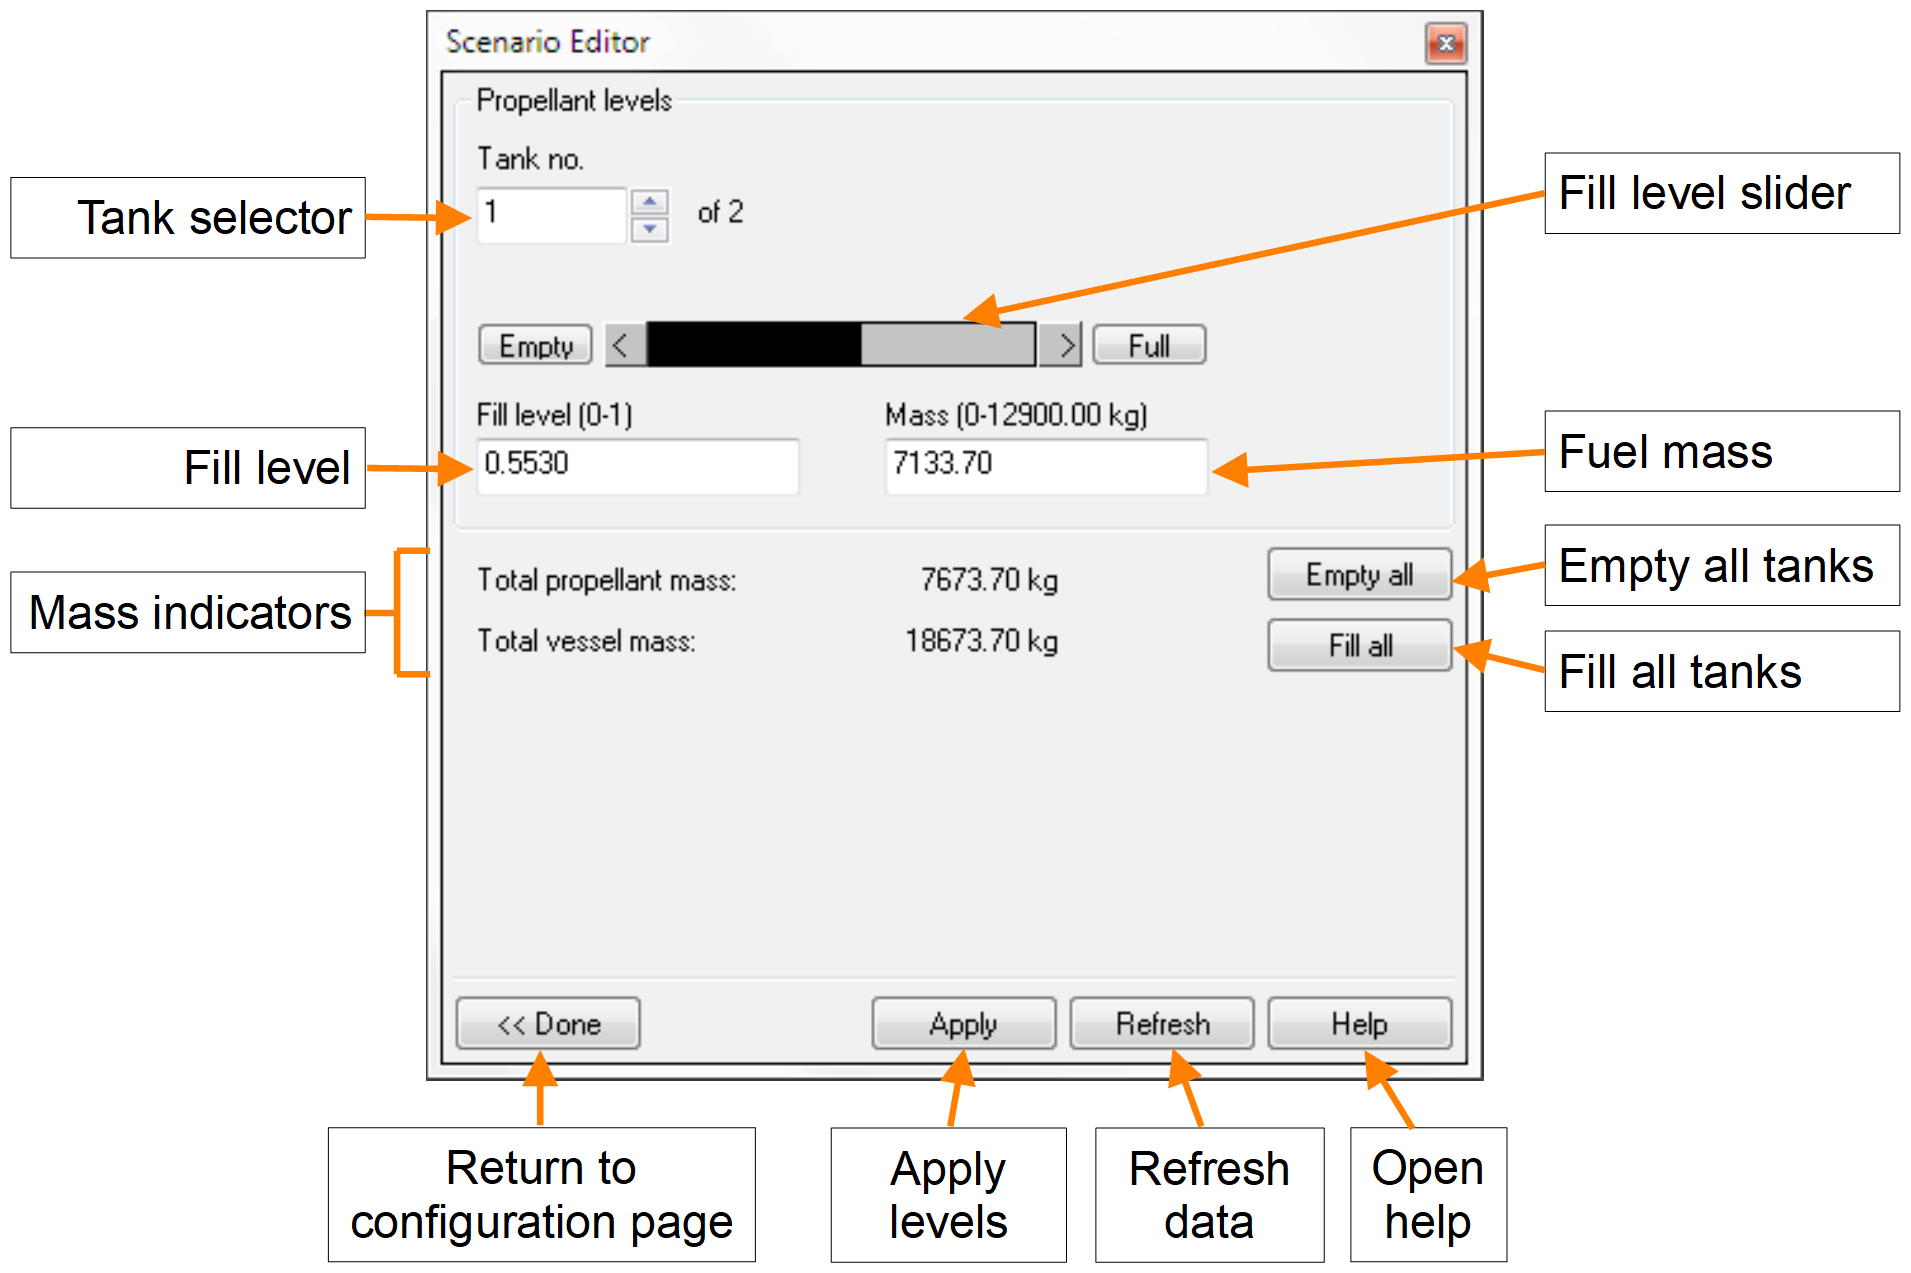
\includegraphics[width=\hsize]{scn_prop.png}
\end{figure}

\subsubsection{Docking management}
If the vessel is equipped with docking ports, this page can be used to set up docking connections to other vessels, or to disengage existing connections.\\
First, select the docking port to operate on. The available docking ports can be cycled with the Dock no. control in the top left. Many spacecraft have only a single docking port, but some - in particular space stations - may have several.\\
Next, an IDS (Instrument Docking System) transmitter can be enabled or disabled for that dock, using the controls in the top right of the page. IDS transmitters allow other vessels to use their Docking MFD and HUD modes for instrument-assisted docking approaches. When IDS is enabled, the transmitter frequency can be adjusted between 108.00-139.95 MHz in 0.05 MHz steps. Make sure that every docking port of the vessel uses a different IDS frequency to avoid interference.\\
Finally, the docking connections at the port can be configured. If a vessel is already docked, its name is displayed. Clicking the \textit{Undock} button breaks the docking connection.\\
If the dock is not engaged, a vessel can be picked from the list provided. Clicking the \textit{Dock} button connects the vessel at the selected dock. If the target vessel has more than one docking port, the connecting port on the target vessel must also be specified.\\
Before executing the docking operation, it is also possible to select how the two vessels are moved to make the connection. The \textit{Bring target to my current position} option will keep the vessel you are configuring at its current position, and drag the target vessel to the docking port of your vessel. The \textit{Move me to current target position} option works in the reverse way: the target vessel maintains its position, and your vessel is dragged to the target vessel's docking port.

\begin{figure}[H]
	\centering
	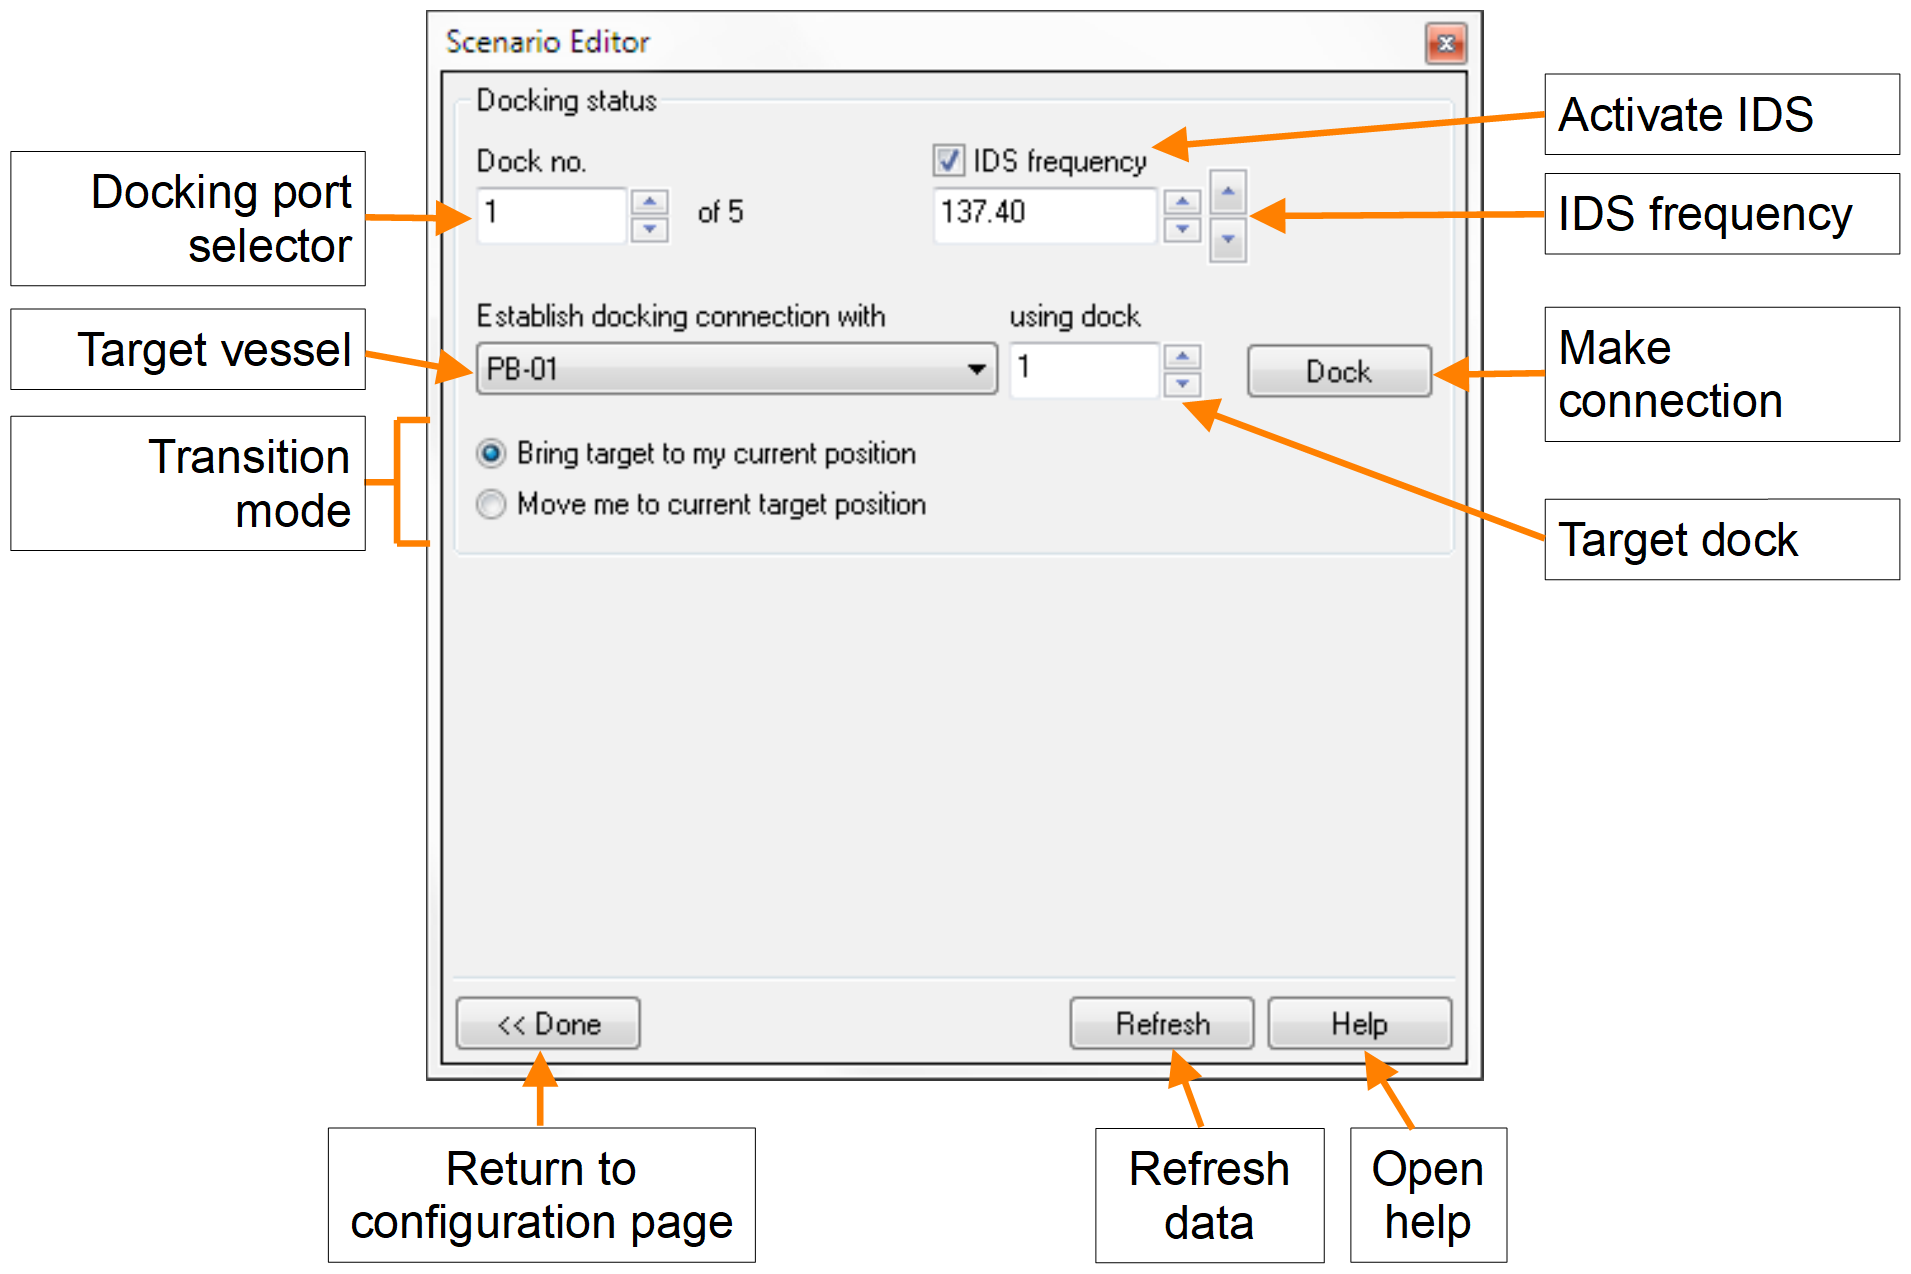
\includegraphics[width=\hsize]{scn_dock.png}
\end{figure}

\noindent
Docking vessels while landed on a planetary surface can sometimes lead to stability problems, in particular if the resulting configuration buries one of the vessels below the surface. See \ref{sssec:scneditor_surface} for a workaround.

\subsubsection{Deleting a vessel}
Clicking the Delete button in the editor's main page deletes the selected vessel. Input focus and camera automatically switch to a different vessel if necessary.\\
You are not allowed to delete all vessels from the simulation: Orbiter requires at least one vessel that accepts control input in a running simulation. Deleting the last vessel leads to undefined behaviour. (Note that some vessels may have been designed not to receive input focus).\\
If the deleted vessel was part of a docked composite structure, the remaining parts of the superstructure will persist in the simulation. If the structure was landed on a planetary surface, the resulting remnant may become instable (try deleting an SRB from a Space Shuttle launch stack!).

\subsubsection{Changing the simulation date and time}
The \textit{Date} button on the editor main page opens the date selection page. It allows to change the date of a running simulation, and specify how vessels are propagated from the current to the new date.\\
The simulation date is displayed in different formats:

\begin{itemize}
\item \textbf{Date and time:} A conventional time specification by day [DD], month [MM], year [YYYY], hour [h], minute [m] and second [s].
\item \textbf{Julian Date (JD):} The interval of time in days and fractions of a day since 1 January 4713 BC, Greenwich noon.
\item \textbf{Modified Julian Date (MJD):} The Julian date minus 2 4000 000.5.
\item \textbf{Julian Century (JC2000):} The interval of time in centuries and fractions of a century since 1 January 2000, Greenwich midnight.
\item \textbf{Epoch:} Year and fraction of a year.
\end{itemize}

\noindent
If any of the date fields are modified, all other date formats are adjusted automatically. Clicking the \textit{Refresh} button updates the dialog fields with the current simulation time. Clicking the \textit{Apply} button sets a new simulation time, and clicking the \textit{Now} button sets the simulation time to the current computer system time. By using the spin controls in the Date and Time section, the simulation time is updated directly.\\
All dates are referenced to Barycentric Dynamical Time (TDB), a common time scale for describing orbital events. TDB is similar to Universal Time (UT), with an offset of currently 66.184 seconds.

\begin{figure}[H]
	\centering
	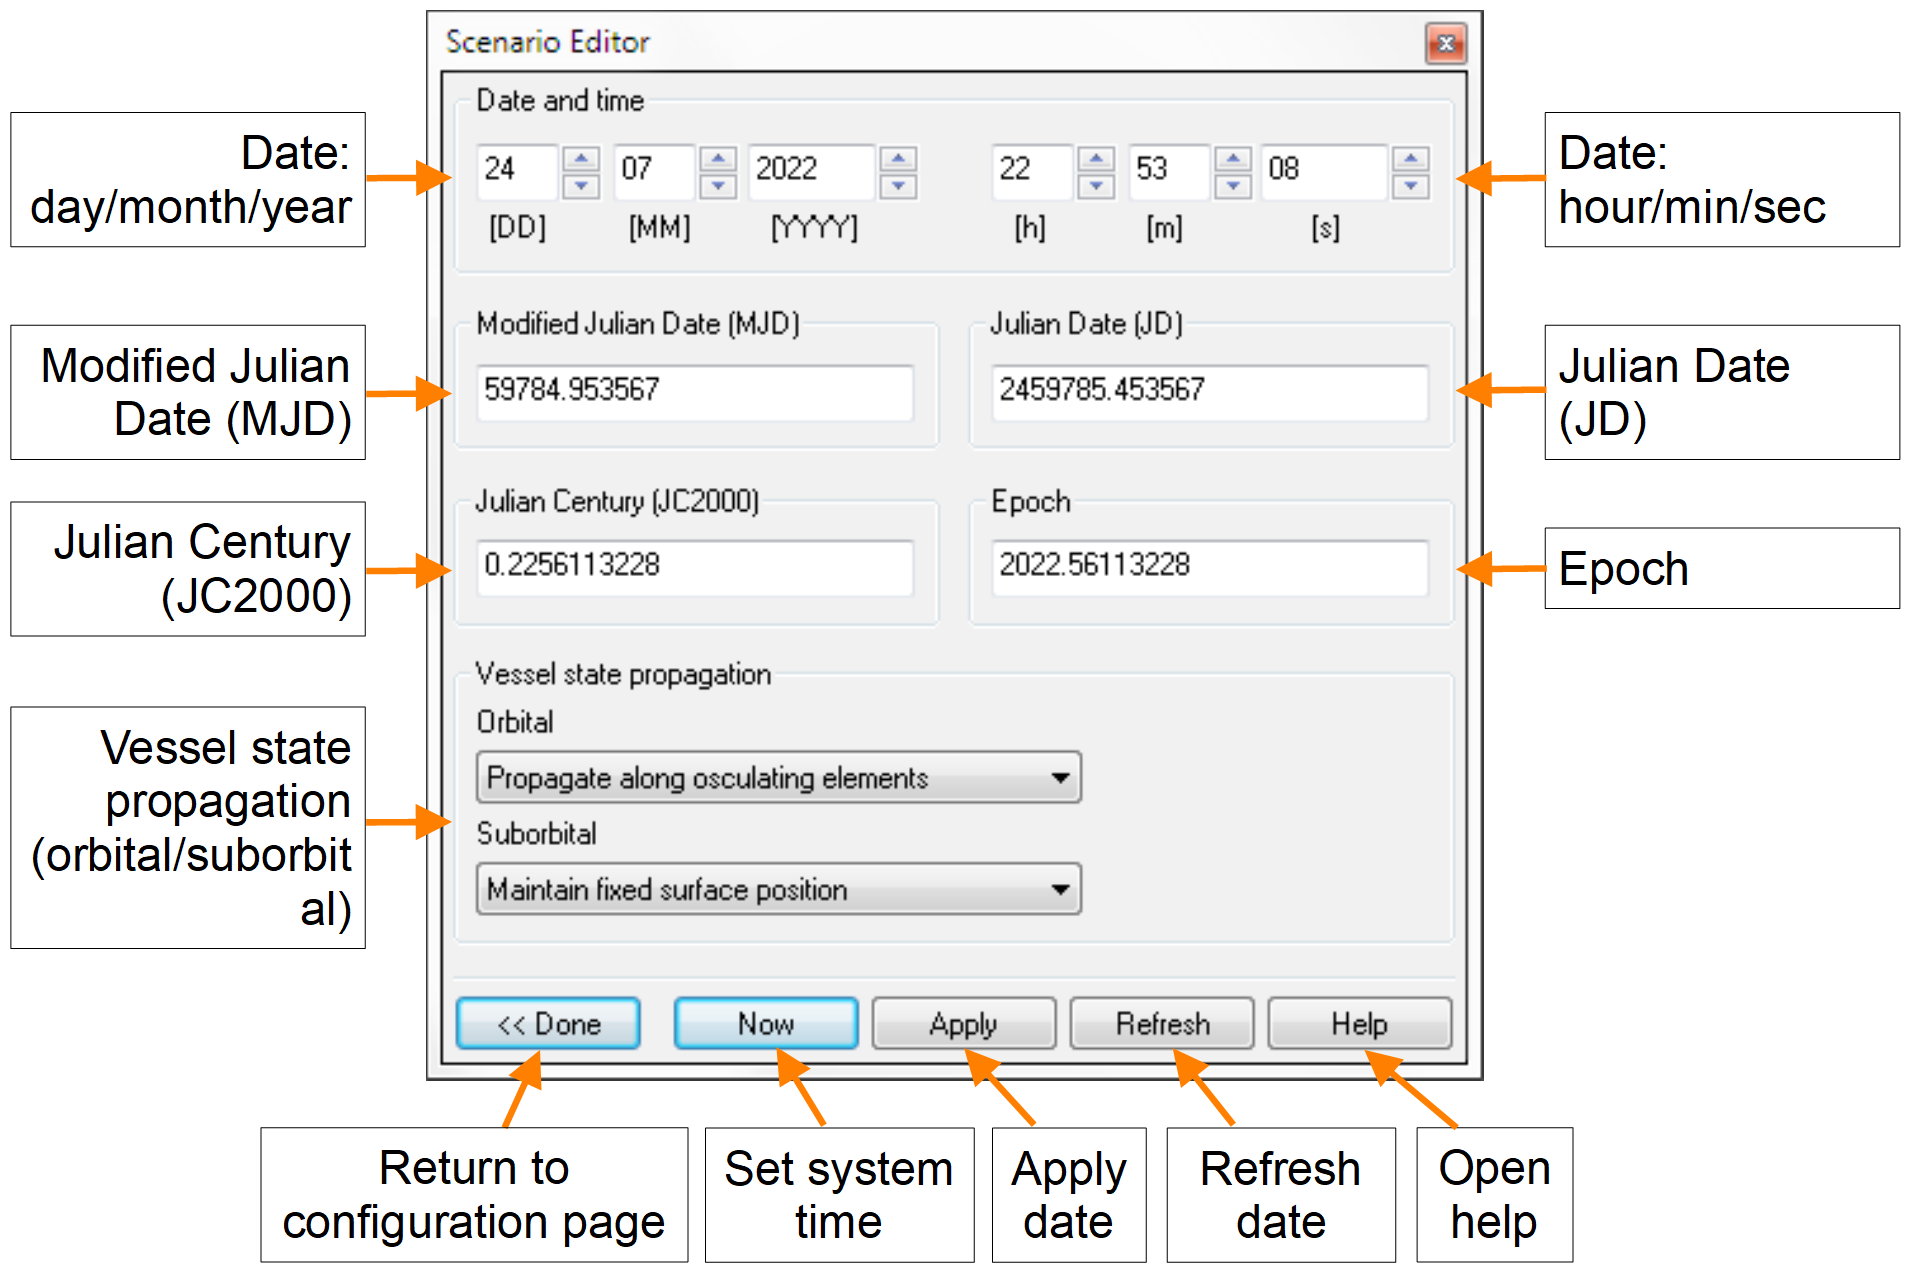
\includegraphics[width=\hsize]{scn_date.png}
\end{figure}

\noindent
Before changing the simulation time, the vessel propagation mode from current to new date should be set. Different propagation modes can be selected for orbiting vessels (with orbits that don't intersect the central body) and for suborbital vessels (with trajectories that intersect the surface). The following options are available for orbital vessels:

\begin{itemize}
\item \textbf{Maintain fixed state vectors:} Keep the vessel's relative position and velocity with respect to the central body fixed in a non-rotating frame. This means that the planet is rotating underneath, while the vessel keeps its location and altitude.
\item \textbf{Maintain fixed surface position:} Keep the vessel's position, velocity and altitude fixed relative to the planet surface. This means that the vessel is rotating together with the planet, and stays fixed above the same point on the surface.
\item \textbf{Propagate along osculating elements:} Move the vessel along its current orbital trajectory, assuming that no forces other than the central body's gravitational force are acting on the vessel.
\end{itemize}

\noindent
For suborbital vessels, in addition to the above one further option is available:

\begin{itemize}
\item \textbf{Destroy vessels:} Destroy any suborbital vessels (i.e. assume that the vessels impacted on the ground during time propagation.
\end{itemize}

\noindent
Time can be adjusted backward as well as forward, but remember that moving back in time will not necessarily restore the simulation to a previous state, because the vessel propagation does not take into account events such as engine burns.

\subsubsection{Saving a scenario}
Once you are happy with the scenario you have created, you can save it to a file which can be run at a later time or shared with other Orbiter users.\\
To save the current simulation state, click the \textit{Save} button on the main editor page. This opens the \textit{Save scenario} page. Enter a file name and a short scenario description. Optionally, the name can include a directory path. All paths are relative to Orbiter's root scenario folder (.\textbackslash Scenarios). The specified directory must already exist.

\begin{figure}[H]
	\centering
	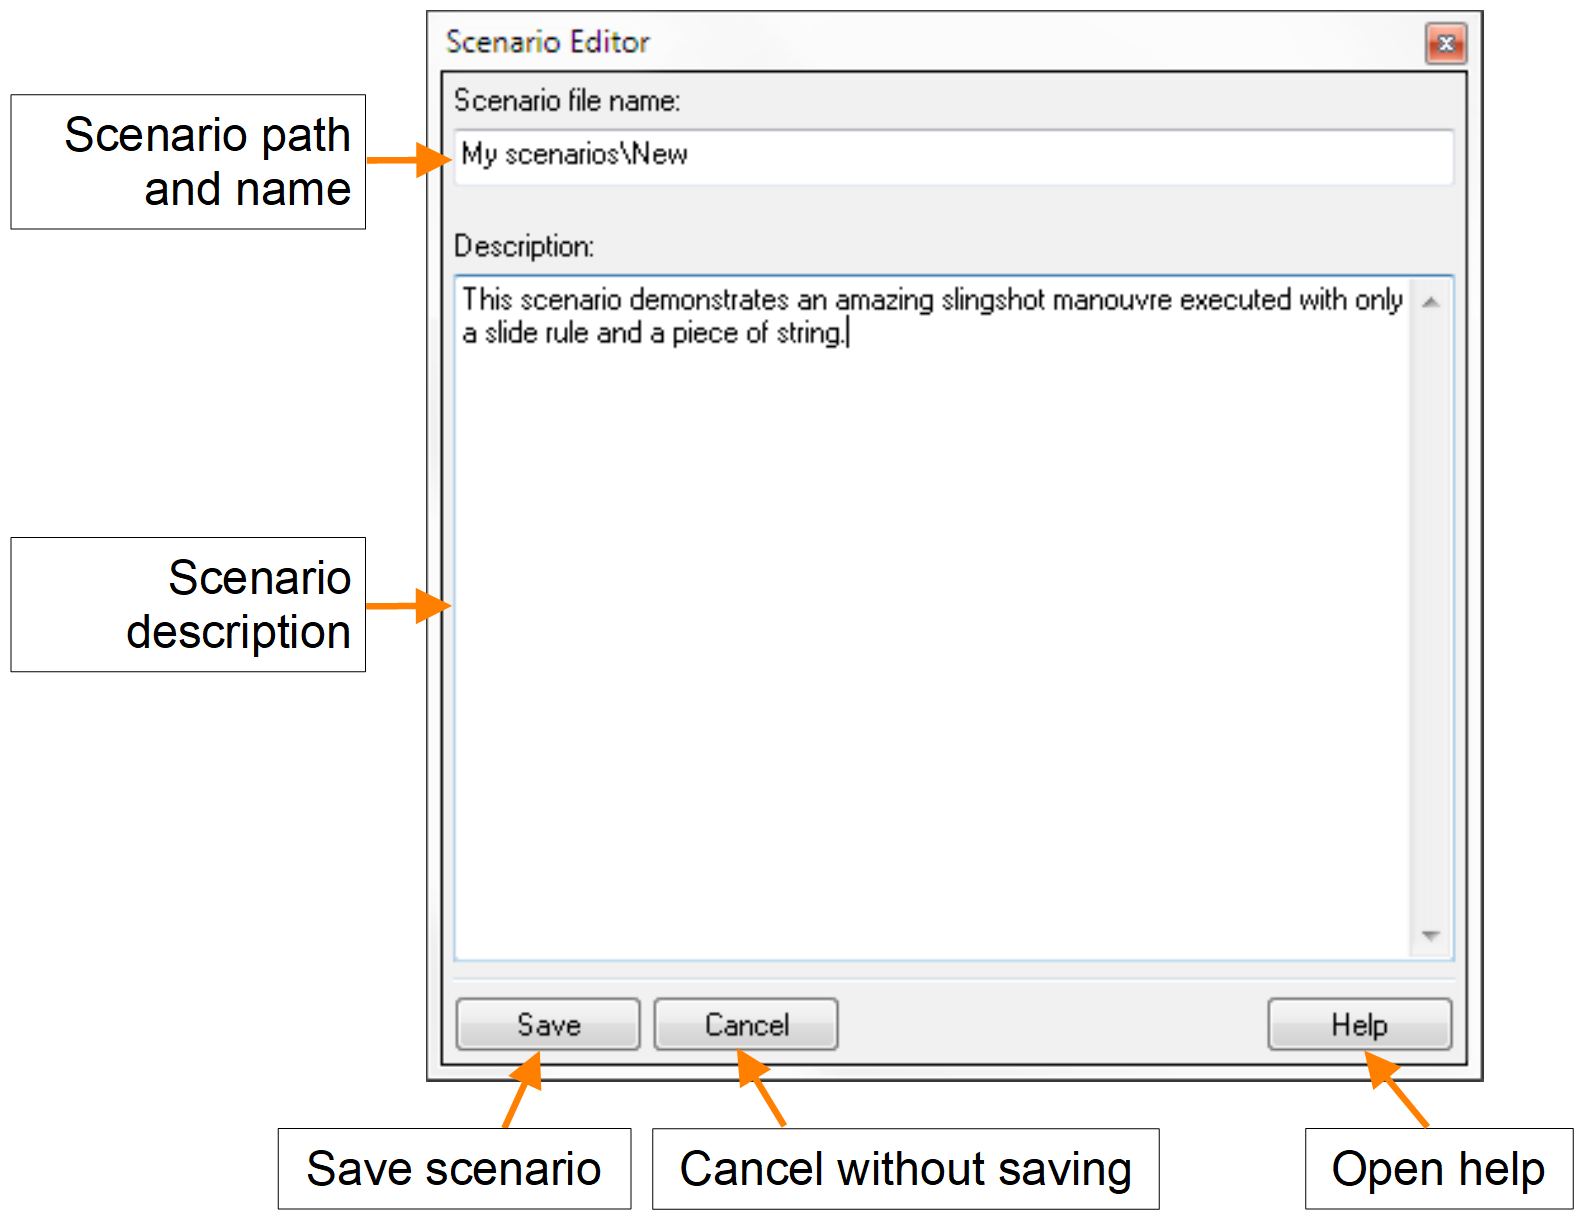
\includegraphics[width=0.8\hsize]{scn_save.png}
\end{figure}

\noindent
The text entered in the description box will be displayed in Orbiter's launchpad dialog when a user selects the scenario from the list. It should briefly explain what the scenario is about.\\
Finally, click \textit{Save} to save the scenario to file, or \textit{Cancel} to return without saving.


\subsection{External MFDs}
If the multifunctional displays (MFD) integrated in the vessel instrument panels do not provide enough information, you can open additional MFD displays in external windows. This is particularly useful in multi-monitor settings where you can display the Orbiter simulation window on one monitor, and a set of MFDs on the other.

\begin{figure}[H]
	\centering
	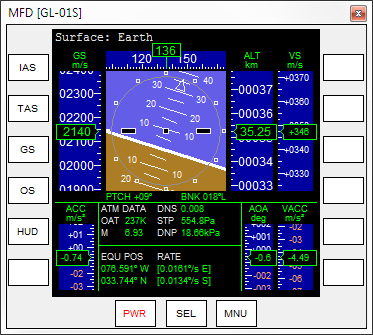
\includegraphics[width=0.4\hsize]{ext_mfd.png}
\end{figure}

\noindent
To open external MFDs, the \textit{ExtMFD} module must be activated in the Orbiter Launchpad dialog. You can then open any number of MFD windows by clicking \textit{External MFD} from the Custom functions dialog (\Ctrl\keystroke{F4}).\\
External MFDs behave in the same way as built-in MFDs. They can be controlled by pressing the buttons around the left, right and bottom edges. See \ref{sec:mfd} for a description of the available MFD modes and controls.\\
Unlike built-in MFD displays, the window MFDs can be resized. They are available in external view as well as cockpit view, and they can be configured to either automatically follow the focus vessel, or remain attached to a specific vessel, even if the focus is switched to a different vessel.


\subsection{Performance meter}
This is a dialog box to keep track of Orbiter's frame rate performance and simulation time step intervals. It shows the frames per second (FPS) and/or the step length interval (in seconds) between consecutive frames in a graphical display over the last 200 seconds. This is a useful tool to estimate the impact of complex scenery and visual effects on the simulation performance. The time step graph also incorporates the effect of time acceleration, and thus reflects the fidelity of the physical model (accuracy of trajectory calculation, etc.)

\begin{figure}[H]
	\centering
	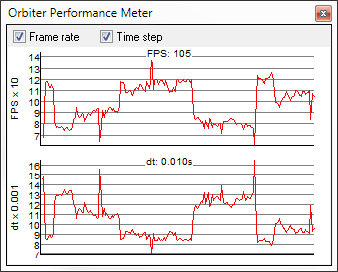
\includegraphics[width=0.4\hsize]{perf_meter.png}
\end{figure}

\noindent
This function is available if the \textit{Framerate} module is active and is accessible via the \textit{Frame Rate} entry in the Custom functions list (\Ctrl\keystroke{F4}).


\subsection{Remote vessel control}
The Remote Vessel Control plug-in allows remote control of the engines of any spacecraft in the simulation.

\begin{figure}[H]
	\centering
	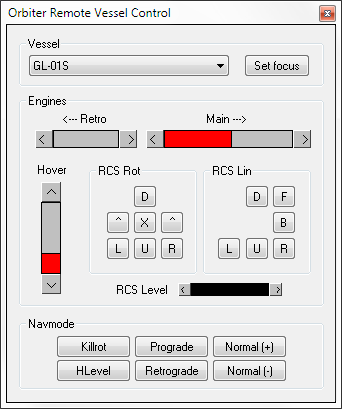
\includegraphics[width=0.4\hsize]{rcontrol.png}
\end{figure}

\noindent
The dialog allows selection of a vessel from a drop-down list. It contains gauges for main, retro and hover engines, controls for RCS thrusters in rotational and linear mode, and provides access to the standard attitude control functions. RCS thrust can be controlled with a slider. This interface can also be useful if simultaneous access to linear and rotational RCS modes is required.\\
This tool is available if the \textit{Rcontrol} module is active and can be accessed via the \textit{Remote Vessel Control} entry in the Custom functions list (\Ctrl\keystroke{F4}).


\subsection{Flight data monitor}
The \textit{Flight data monitor} graphically displays a number of flight parameters as a function of time. This tool is available if the \textit{FlightData} module is active. The dialog box is accessible via the Custom functions list (\Ctrl\keystroke{F4}).

\begin{figure}[H]
	\centering
	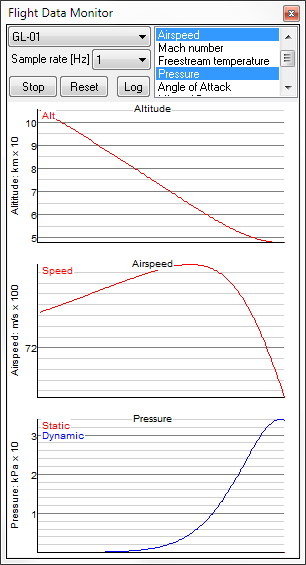
\includegraphics[width=0.3\hsize]{flight_data_monitor.png}
\end{figure}

\noindent
The control area of the dialog box allows selection of the vessel for which data are displayed, sampling rate, and the set of data to show.\\
The following parameter displays are supported:

\begin{itemize}
\item Altitude
\item Airspeed
\item Mach number
\item Free stream temperature
\item Static and dynamic pressure
\item Angle of attack
\item Lift and drag force
\item Lift over drag ratio (L/D)
\item Vessel mass
\end{itemize}

\noindent
For each parameter category selected in the list, a graph display is opened below the control area to track that parameter as a function of time.

\begin{itemize}
\item The Start/Stop button starts or stops the update of the data graphs.
\item The Reset button clears the data graphs.
\item The Log button starts or stops the output of flight data to a log file. When the Log button is ticked, Orbiter writes out data into text file FlightData.log in the main Orbiter directory. This file can later be used to analyse or visualise the data with external tools. FlightData.log is overwritten whenever Orbiter is restarted.
\end{itemize}


\subsection{Lua Console}
\label{ssec:lua_console}
The \textit{Lua Console} window is available from the Custom functions list (\Ctrl\keystroke{F4}) if the \textit{LuaConsole} module has been activated. The console provides an interactive script interface which allows script execution (tutorials, autopilots, etc.) and reading/writing of simulation and spacecraft parameters and states. The script interface and Orbiter Lua extensions are described in more detail in \ref{sec:script}.

\begin{figure}[H]
	\centering
	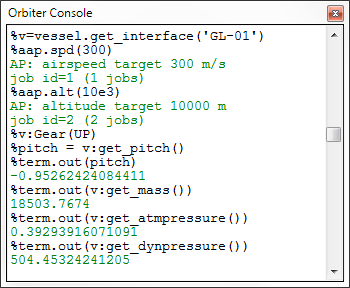
\includegraphics[width=0.4\hsize]{console.png}
\end{figure}


\subsection{Draw Orbits}
\infobox{This plug-in is only available in the D3D9 graphics client.}

\noindent
The DrawOrbits plug-in draws a line along the path of orbit of the vessel in focus, allowing the user to have a visual representation of the current orbit around a celestial body. In addition, it indicates the location of the apoapsis and periapsis, as well as the ascending and descending nodes.\\
Listed at each apsis is the time to reach it and altitude above surface, and shown at the nodes is the orbital inclination and longitude of the ascending node, in relation to the ecliptic.

%TODO update image when degree sign is fixed
\begin{figure}[H]
	\centering
	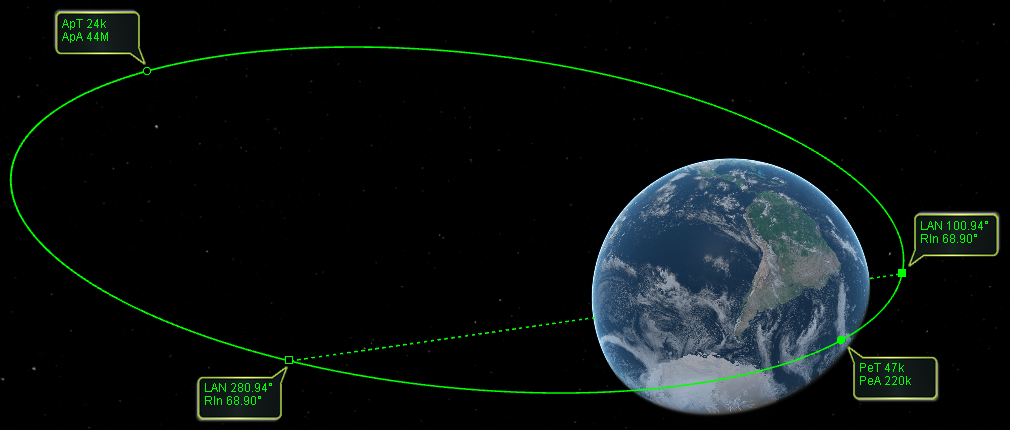
\includegraphics[width=0.99\hsize]{draworbits_vessels.png}
	\caption{Orbit of a vessel around Earth.}
\end{figure}

\noindent
The orbits of the celestial bodies are also drawn, ilustrating the different orbits of the moons around planets.

\begin{figure}[H]
	\centering
	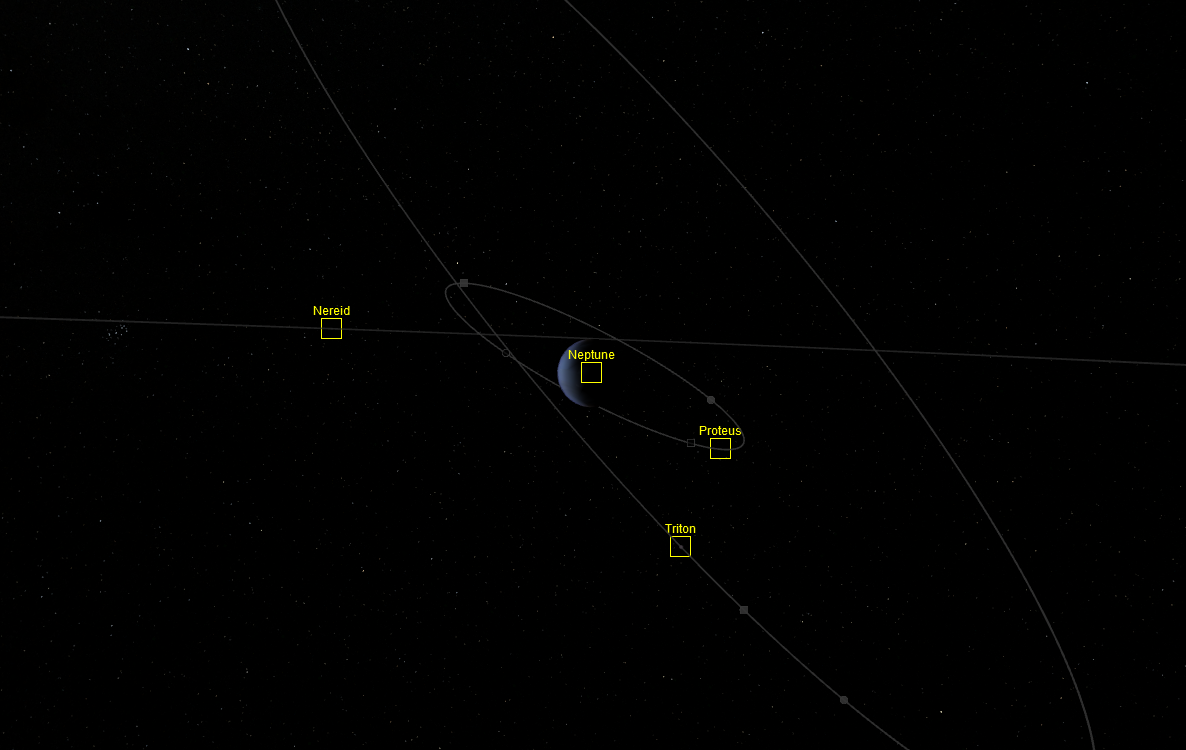
\includegraphics[width=0.99\hsize]{draworbits_bodies.png}
	\caption{Visualisation of the orbits of 3 moons around Neptune.}
\end{figure}


\end{document}
